\documentclass[a4paper, 12pt, titlepage]{article}

% \usepackage{amsfonts}
\usepackage{amsmath}
\usepackage{amssymb}
\usepackage{bytefield}
% \usepackage{caption}
\usepackage{fancyhdr}
\usepackage[left=2.5cm, right=2.5cm]{geometry} % for better on-line reading
\usepackage{float}
% \usepackage{graphicx}
\usepackage{hyperref}
\usepackage{lastpage}
\usepackage{lettrine}
% \usepackage{listings}
\usepackage{lmodern}
% \usepackage{makeidx}
% \usepackage{placeins}
\usepackage{setspace}
\usepackage{subcaption}
% \usepackage{textcomp}
\usepackage{titlesec}
\usepackage{titling}
\usepackage[dvipsnames]{xcolor}

\usepackage[backend=biber, style=alphabetic]{biblatex}
\addbibresource{bibliography.bib}

\usepackage{pgfplots}
\pgfplotsset{compat=1.16}

\usepackage{tikz}
\usetikzlibrary{shapes,arrows,calc,fit,positioning}

\input Acorn.fd
\newcommand*\initfamily{\usefont{U}{Acorn}{xl}{n}}

% colors
\definecolor{royalblue}{cmyk}{1,0.50,0,0}
\definecolor{nemdark}{HTML}{44004E}
\definecolor{nemleading}{HTML}{5200c6}
\definecolor{nemorange}{HTML}{ff9600}
\definecolor{nemgreen}{HTML}{33dd50}


% page formatting and footer
\pagestyle{fancy}
\fancyhf{}
\cfoot{Page \thepage \hspace{1pt} of \pageref{LastPage}}

% title formatting
\titleformat{\section}
{\color{nemleading}\normalfont\Large\bfseries}
{\color{nemorange}\thesection}{1em}{}

% paragraph formatting
\setlength{\parskip}{2.5mm}
\setlength{\parindent}{4mm}

% hyperlink formatting
\hypersetup{
	colorlinks,
	linkcolor={cyan!60!black},
	citecolor={blue!50!black},
	urlcolor={blue!80!black}
}

% blue node
\tikzset{fontscale/.style = {font=\small}}
\tikzstyle{cblue}=[circle, draw, thin, fill=cyan!10, scale=0.2, align=center, fontscale=4]

% transparent node
\tikzstyle{ctra}=[rectangle, thin]
\tikzstyle{crou}=[rectangle, draw, rounded corners, thin]
\tikzstyle{crecb}=[rectangle, draw, thin, text height=12pt,text depth=5pt,solid,rounded corners=0]
\tikzstyle{legend_phytop}=[rectangle, draw, rounded corners, thin,
	minimum width=2.5cm, minimum height=0.8cm,
	royalblue
]
\tikzstyle{legend_normal}=[rectangle]

\pretitle{
	\begin{center}
	
\includegraphics{images/NEM_wankel_round.pdf}
	\\
	\vspace{15mm}
}

\title{
	\fontsize{72pt}{74pt}\textbf{NEM}
	\\
	\vspace{5mm}
	\fontsize{18pt}{20pt}\textit{技术指南(白皮书)}
	\\
	\vspace{20mm}
	\fontsize{12pt}{14pt}{版本 1.0}
}
\author{}
\date{1月2日,2020年}

% % nem index
% \newcommand{\nind}[1]{
% 	\emph{#1}\index{#1}
% }

% % transaction index - less typing
% \newcommand{\tind}[1]{
% 	\emph{#1 transaction}\index{transaction!\lowercase{#1}}
% }

% \newcommand{\nemref}[1]{
% 	\autoref{#1}:~\nameref{#1}
% }

\newcommand{\nemchapterfirstletter}[1]{
	\lettrine[lraise=0,lines=4,nindent=0.5em,slope=0.0em]{\initfamily\color{nemgreen}\fontsize{72pt}{74pt}\selectfont #1}
}

%%% quote formating %%%

% selects Libertine for quote font
\newcommand*\quotefont{
	\fontfamily{LinuxLibertineT-OsF}
}

\newcommand*{\openquote}{
	\tikz[remember picture,overlay,xshift=-15pt,yshift=10pt]
	\node[] (OQ) {\quotefont\fontsize{60}{60}\selectfont``};
	\kern0pt
}
\newcommand*{\closequote}{
	\tikz[remember picture,overlay,xshift=15pt,yshift=0pt]
	\node[] (CQ) {\quotefont\fontsize{60}{60}\selectfont''};
}

\newcommand{\nemquote}[2]{
	\begin{quote}\openquote #1 \hfill\closequote
	\par \hfill \textit{- #2}
	\end{quote}
}

% 本文件将对中文的样式和命令进行配置和定义


\makeindex[intoc]
\renewcommand{\contentsname}{目录}

\begin{document}
\pagenumbering{roman}

	\phantomsection\pdfbookmark[section]{\codename}{titlepage}

\begin{CJK}{UTF8}{gbsn}
	\begin{titlepage}
	\maketitle
	\end{titlepage}
	\phantomsection\pdfbookmark[section]{\contentsname}{toc}

	\pagestyle{empty}
	\setcounter{page}{2}

	\begin{spacing}{0}
	{
		\pagestyle{empty}
		\fancypagestyle{plain}{
			\fancyhf{}
			\renewcommand{\headrulewidth}{0pt}
			\renewcommand{\footrulewidth}{0pt}
		}
		\pagenumbering{roman}
		\pagestyle{empty}
		\tableofcontents
		\thispagestyle{empty}
		{
		\pagestyle{empty}
		\refstepcounter{section}
\section*{Typographical Conventions}
\addcontentsline{toc}{section}{Typographical Conventions}

\begin{table}[ht]
	\nemcenterwithcaption{
		\begin{tabular}{|p{0.45\linewidth}|p{0.20\linewidth}|p{0.25\linewidth}|}
			\hline
			\textbf{Description} & \textbf{Attributes} & \textbf{Example} \\
			\hline
			Project name & bold, colored & \codename \\
			\hline
			Classes & fixed-width font & \class{ProcessBootstrapper} \\
			\hline
			Fields & fixed-width font & \field{FeeMultiplier} \\
			\hline
			File paths & fixed-width font & \filepath{commit\_step.dat} \\
			\hline
			Configuration settings (prefixed with configuration filename) in text mode & italic & \nemsetting{network}{maxDifficultyBlocks} \\
			\hline
			Configuration settings (without configuration filename) in equations and formulas & regular & $\nemsetting{network}{maxDifficultyBlocks}$  \\
			\hline
			Fields in equations and formulas & regular & $\structField{T}{SignerPublicKey}$ \\
			\hline
			Function names in equations and formulas & regular & $\mathfunc{VerifiableDataBuffer}()$ \\
			\hline
		\end{tabular}
	}{Typographical conventions used in this document}
\end{table}

	}
	}
	\end{spacing}

	\refstepcounter{section}
\section*{前言}
\addcontentsline{toc}{section}{前言}

\nemquote{
你错过了100\%的你没有尝试的击球机会。
}{韦恩·格雷茨基\footnote{韦恩·格雷茨基,加拿大的职业冰球明星。}}

NEM最初的起源是在2014年1月bitcointalk论坛中一篇帖子里的“投名状”。
加密数字货币领域刚刚经历了2013年底的一波爆发,尽管当时的价格与数年之后相去甚远,可这时的人们总是充满了热情。
NXT主网的发布使得其成为了最早期的POS区块链之一,NEM的早期社区从中汲取了灵感和人才,其中就包括了三位至今仍活跃着的核心研发者。

最初有很多关于我们要做什么的讨论,但我们很快决定要从零开始做一些全新的东西。
This allowed for more design flexibility as well as the use of high coding standards from the very beginning.
This also gave us the opportunity to contribute something new to the blockchain landscape.
我们想要挑战自己,看看能不能做出什么有用的产品来。
作为很多个周末跟夜晚辛勤付出的结果,我们终于在2015年的3月份发布了名为NIS1的NEM主网。
我们对于这个产品感到很满意,但是我们清楚在开发的过程中也采取了一些捷径,于是我们决定继续改善它。
最终,我们意识到了原先解决方案需要一次技术重构来突破核心性能瓶颈,同时适应未来更快速的创新。

我们非常感激TechBureau对我们从零开始创建一条全新的链的支持 - \codename.
我们希望这些条新的链可以解决NIS1存在的众多问题,并且为未来的性能增强和发展提供坚实的基础。
我们的使命是创建一个高性能的“区块链”,而非基于DAG或是dBFT的系统。
在这种意义上而言,我们认为,我们是成功的。

这对于我们来说是一个漫长的旅程,我们希望这是最后一条我们从零开始构建的区块链。
This has been a long journey for us, but we are excited to see what yet is to come and what novel things \textbf{you} use \codenamespace to build.
我们对于未来感到兴奋,也期待看到你们使用\codenamespace创建的全新产品。
最后,再次感谢给予那些我们灵感和支持的人们\ldots

\begin{flushright}
BloodyRookie
gimre
Jaguar0625
\end{flushright}

	\refstepcounter{section}
\section*{Typographical Conventions}
\addcontentsline{toc}{section}{Typographical Conventions}

\begin{table}[ht]
	\nemcenterwithcaption{
		\begin{tabular}{|p{0.45\linewidth}|p{0.20\linewidth}|p{0.25\linewidth}|}
			\hline
			\textbf{Description} & \textbf{Attributes} & \textbf{Example} \\
			\hline
			Project name & bold, colored & \codename \\
			\hline
			Classes & fixed-width font & \class{ProcessBootstrapper} \\
			\hline
			Fields & fixed-width font & \field{FeeMultiplier} \\
			\hline
			File paths & fixed-width font & \filepath{commit\_step.dat} \\
			\hline
			Configuration settings (prefixed with configuration filename) in text mode & italic & \nemsetting{network}{maxDifficultyBlocks} \\
			\hline
			Configuration settings (without configuration filename) in equations and formulas & regular & $\nemsetting{network}{maxDifficultyBlocks}$  \\
			\hline
			Fields in equations and formulas & regular & $\structField{T}{SignerPublicKey}$ \\
			\hline
			Function names in equations and formulas & regular & $\mathfunc{VerifiableDataBuffer}()$ \\
			\hline
		\end{tabular}
	}{Typographical conventions used in this document}
\end{table}


	\setcounter{section}{0}
	\renewcommand*{\theHsection}{body\the\value{section}}


	\pagestyle{fancy}
	\pagenumbering{arabic}
	\setcounter{page}{1}

	\section{引言}
\label{sec:introduction}

\nemquote{
于灰烬中唤醒火焰,
于阴影中焕发光明;
折断的利刃将重露锋芒,
那无冕之人将重新称王。
}{J.R.R. 托尔金\footnote{J.R.R.托尔金,英国作家,诗人,著有《魔戒》系列。}}

基于区块链的去信任,高性能,分层体系结构的DLT协议-这些是影响\codename 研发的首要原则。
尽管考虑了其他DLT协议,包括DAG和dBFT,但很快就选择了区块链作为最符合去信任的理想协议。
任何节点都可以下载区块链的完整副本,并且可以随时独立进行验证。
具有足够收获能力的节点总是可以创建块,而无需依赖领导者。
这些选择必然会牺牲一些相对于其他协议的吞吐量,但它们似乎与比特币的哲学基础最一致。\cite{nakamoto2009}.

作为聚焦去信任的一部分,在NEM的基础上添加了以下功能:
\begin{itemize}
    \item{可以在没有事务数据的情况下同步块头,同时允许验证链的完整性}
    \item{交易merkle树允许在区块内对交易是否存在进行加密证明}
    \item{收据增加了间接触发状态更改的透明度}
    \item{状态证明允许对区块链中的特定状态进行去信任验证}
\end{itemize}


在\codename中,有一个单一服务器可执行文件,可以通过加载不同的插件(用于事务支持)和扩展名(用于功能性)进行自定义。
(每个网络)有三种主要配置,但是通过启用或禁用特定扩展,可以进一步定制混合配置。

三种主要配置是:
\begin{enumerate}
\item Peer:Peer节点是网络的主心骨,他们会产出新的块。
\item API: API节点将数据存储在mongo数据库中,以便于查询,并且可以与NodeJS REST服务器结合使用。
\item Dual: Dual节点同时具有Peer节点和Api节点的功能。
\end{enumerate}


一个强大的网络通常将具有大量的Peer节点和足够的API节点来支持传入的客户端请求。
允许节点的组成根据实际需求动态变化,应该网络的资源全局更加优化。

相对于典型的区块链协议,以干扰器(Disruptor)模式为基础的核心区块和事务流水线-并尽可能使用并行处理-可以实现每秒较高的事务速率。


NIS1是值得记录在区块链领域的技术,\codenamespace是其更有价值的演变。
这不是结束,而仅仅是新的开始。
我们还有更多工作要做。

\subsection{变种}

\codenamespace 支持其主要哈希算法的编译时间替换,该算法从输入数据中生成32字节的值。
为简洁起见,本文档的其余部分将在假定其默认设置(SHA3)的情况下引用此哈希。
当前,支持以下哈希算法:

\begin{enumerate}
    \item{SHA3 (default): SHA3是默认模式,建议新的链采用。}
    \item{Keccak: 提供此模式是为了与诸如NIS1之类的旧式链兼容,以便保留私钥:公钥:地址之间的映射。}
\end{enumerate}

	\section{系统}
\label{sec:system}

\nemquote{
}{}


\codenamespace在网络级别和单个节点级别都支持高度的自定义。
\nemsetting {network} {network}中指定的网络范围设置对于网络中的所有节点必须相同。
\nemsetting {node} {node}中指定的特定于节点的设置在同一网络中的各个节点之间可能会有所不同。
\codenamespace was designed to use a \emph{plugin / extension} approach instead of supporting Turing complete smart contracts.
While the latter can allow for more user flexibility, it's also more error prone from the user perspective.
A plugin model limits the operations that can be performed on a blockchain and consequently has a smaller attack surface.
Additionally, it's much simplier to optimize the performance of a discrete set of operations than an infinite set.
This helps \codenamespace achieve the high throughput for which it was designed.

\subsection{事务插件}


网络中的所有节点必须支持相同类型的事务,并以完全相同的方式处理它们,以便所有节点可以就全局区块链状态达成共识。
网络事务由一组网络需要每个节点都需要加载的\emph{transaction plugins}\index{plugins}来支持。
这个(事务插件)组是由存在\nemsetting{network}{network} 配置部分。
这些插件的任何更改,添加或删除必须由所有网络节点协调并接受。
如果仅节点的部分子集同意这些修改,则这些节点将在分叉上。
\codenamespace所有内置的事务都使用此插件模型构建,以验证其可扩展性。

插件是一个单独的动态链接库,它以以下形式开放单个接口
\footnote{插件的格式取决于目标操作系统和使用的编译器,因此所有主机应用程序和插件必须使用相同的编译器版本和选项构建。}:

\begin{lstlisting}
extern "C" PLUGIN_API
void RegisterSubsystem(
	catapult::plugins::PluginManager& manager);
\end{lstlisting}

\class{PluginManager} 类提供对插件初始化所需的配置子集的访问。
通过这个类,插件可以注册以下零个或多个:

\begin{enumerate}
	\item{事务(Transaction) -
		可以指定新的事务类型以及这些类型到解析规则的映射。
		具体来说,该插件定义了将交易转换为组件通知的规则,这些通知将在进一步处理中使用。
		还可以指定一些处理约束,例如指示事务只能出现在聚合事务中\nemrefparens{sec:transactions:aggregate}。
	}
	\item{缓存(Caches) -
		可以指定新的缓存类型和规则,以将模型类型与二进制进行序列化和反序列化。
		启用该功能后,可以选择将每个与状态相关的缓存包括在块的\field{StateHash}\nemrefparens{sec:blocks:statehash}的计算中。
	}
	\item{联络程序(Handlers) - 总是可以访问的APIs。}
	\item{诊断器(Diagnostics) - 仅当节点以诊断方式运行时才可访问的API和计数器。}
	\item{验证器(Validators) -
		无状态和有状态验证器,用于处理由区块和事务处理产生的通知。
		经过注册的验证器可以订阅常规或插件定义的通知,并拒绝不允许的值或状态更改。	
	}
	\item{监察器(Observers) -
		监察器处理由区块和事务处理产生的通知。
		经过注册的监察器可以订阅常规或插件定义的通知,并根据其值更新区块链状态。
		监察器不需要任何验证逻辑,因为只有在所有适用的验证者成功之后才调用监察器。
	}
	\item{解析器(Resolvers) -
		可以指定从未解析类型到已解析类型的自定义映射。
		例如,名称空间插件使用它来添加对别名(Alias)解析的支持。
	}
\end{enumerate}

\subsection{\codenamespace 扩展}
\label{sec:system:extensions}

允许网络内的各个节点支持功能的异构混合。
例如,某些节点可能希望将数据存储在数据库中或将事件发布到消息队列。
这些功能都是可选的,因为它们都不影响共识。
此类功能由节点加载的\emph{extensions}集确定,如\nemsetting{extensions-\{process\}}{extensions}中指定的那样。
大多数内置\codenamespace功能是使用此扩展模型构建的,以验证其可扩展性。

扩展是一个单独的动态链接库,它以以下形式开放单个接口
\footnote{扩展的格式取决于目标操作系统和所使用的编译器,因此所有主机应用程序和插件必须使用相同的编译器版本和选项来构建。}:

\begin{lstlisting}
extern "C" PLUGIN_API
void RegisterExtension(
	catapult::extensions::ProcessBootstrapper& 
	bootstrapper);
\end{lstlisting}

\class{ProcessBootstrapper} 类提供对扩展名自行初始化的完整\codenamespace配置和服务的访问。
提供此附加访问权限使扩展比插件更强大。
通过此类,扩展可以注册以下零个或多个:

\begin{enumerate}
	\item{服务(Services) -
		服务代表独立的行为。
		服务传递了一个表示可执行文件状态的对象,并且可以使用它来配置多种事物。
		服务尤其可以添加诊断计数器,定义API(诊断和非诊断API)并将任务添加到任务计划程序。
		它还可以创建从属服务,并将其生存期与托管可执行文件的生存期相关联。
		服务的功能几乎没有限制,这允许进行重大定制化开发。
	}
	\item{订阅(Subscriptions) -
		扩展可以订阅任何受支持的区块链事件。
		检测到更改时会引发事件。
		支持阻止,状态,未确认的事务和部分事务更改事件。
		事务处理完成时,将引发事务状态事件。
		发现远程节点时会引发节点事件。
	}
\end{enumerate}

除上述内容外,扩展还可以更复杂的方式配置节点。
例如,分机可以注册自定义网络时间源。
实际上,有一个专门的扩展程序可以根据\nemref{sec:timesync}中描述的算法建立时间源。
这是此扩展模型允许的高级别定制的一个示例。
要了解扩展所允许的全部扩展性,请参阅项目代码或开发人员文档。\nemtechdocsfootnote{}.

\subsection{服务器}

最简单的\codenamespace拓扑由单个服务器可执行文件组成。
网络和\codenamespace所需的事务插件节点操作员所需的扩展由服务器加载和初始化。

\codenamespace 将其所有数据存储在 \filepath{data} 目录(directory)中。
数据目录的内容如下:

\begin{enumerate}
	\item{区块版本目录(Block Versioned Directories) -
		这些目录包含专有格式的区块信息。
		每个已确认区块的二进制数据,事务记录和相关数据都存储在这些目录中。
		处理每个块时生成的语句 \nemrefparens{sec:blocks:receipts}也存储在此处以便快速访问。
		版本化目录的一个示例是 \filepath{00000},它包含第一组块。
	}
	\item{\filepath{audit} - Audit files created by the audit consumer \nemrefparens{sec:disruptor:commonConsumers} are stored in this directory.}
	\item{\filepath{spool} -
		Subscription notifications are written out to this directory.
		They are used as a message queue to pass messages from the server to the broker.
		They are also used by the recovery process to recover data in the case of an ungraceful termination.
	}
	\item{\filepath{state} -
		\codenamespace stores its proprietary storage files in this directory.
		\filepath{supplemental.dat} and files ending with \filepath{\_summary.dat} store summarized data.
		Files ending in \filepath{Cache.dat} store complete cache data.
	}
	\item{\filepath{statedb} - When \nemsetting{node}{enableCacheDatabaseStorage} is set, this directory will contain RocksDB files.}
	\item{\filepath{transfer\_message} -
		When \nemsetting{user}{enableDelegatedHarvestersAutoDetection} is set, this directory will contain extracted delegated harvesting requests for the current node.
	}
	\item{\filepath{commit\_step.dat} -
		This stores the most recent step of the commit process initiated by the server.
		This is primarily used for recovery purposes.
	}
	\item{\filepath{index.dat} - This is a counter that contains the number of blocks stored on disk.}
\end{enumerate}

\subsubsection{Cache Database}

The server can run with or without a cache database.
When \nemsetting{node}{enableCacheDatabaseStorage} is set, RocksDB is used to store cache data.
Verifiable state \nemrefparens{sec:blocks:statehash} requires a cache database and most network configurations are expected to have it enabled.

A cache database should only be \emph{disabled} when all of the following are true:

\begin{enumerate}
	\item{High rate of transactions per second is desired.}
	\item{Trustless verification of cache state is not important.}
	\item{Servers are configured with a large amount of RAM.}
\end{enumerate}

In this mode, all cache entries are always resident in memory.
On shutdown, cache data is written to disk across multiple flat files.
On startup, this data is read and used to populate the memory caches.

When a cache database is enabled, summarized cache data is written to disk across multiple flat files.
This summarized data is derivable from data stored in caches.
One example is the list all high-value accounts that have a balance of at least \nemsetting{network}{minHarvesterBalance}.
While this list can be generated by (re)inspecting all accounts stored in the account state cache, it is saved to and loaded from disk as an optimization.

\subsection{Broker}

The broker process allows more complex \codenamespace behaviors to be added without sacrificing parallelization.
Transaction Plugins required by the network and \codenamespace Extensions desired by the node operator are loaded and initialized by the broker.
Although the broker supports all features of Transaction Plugins, it only supports a subset of \codenamespace Extensions features.
For example, overriding the network time supplier in the broker is not supported.
Broker extensions are primarily intended to register subscribers and react to events forwarded to those subscribers.
Accordingly, it's expected that the server and broker have different extensions loaded.
Please refer to the project code or developer documentation for more details.

The broker monitors the \filepath{spool} directories for changes and forwards any event notifications to subscribers registered by loaded extensions.
Extensions register their subscribers to process these events.
For example, a database extension can read these events and use them to update a database to accurately reflect the global blockchain state.

\filepath{spool} directories function as one way message queues.
The server writes messages and the broker reads them.
There is no way for the broker to send messages to the server.
This decoupling is intentional and was done for performance reasons.

The server raises subscription events in the blockchain sync consumer \nemrefparens{sec:disruptor:blockConsumers} when it holds an exclusive lock to the blockchain data.
These operations are offloaded to the broker to prevent slow database operations when the server has an exclusive lock.
The server overhead is minimal because most of the data used by the broker is also required to recover data after an ungraceful server termination.

\subsection{Recovery}

The recovery process is used to repair the global blockchain state after an ungraceful server and/or broker termination.
Transaction Plugins required by the network and \codenamespace Extensions desired by the node operator are loaded and initialized by the recovery process.
When a broker is used, the recovery process must load the same extensions as the broker.

The specific recovery procedure depends on the process configuration and the value of the \filepath{commit\_step.dat} file.
Generally, if the server exited after state changes were flushed to disk, those changes will be reapplied.
The blockchain state will be the same as if the server had applied and committed those changes.
Otherwise, if the server exited before state changes were flushed to disk, pending changes will be discarded.
The blockchain state will be the same as if the server had never attempted to process those changes.

After the recovery process completes, the blockchain state should be indistinguishable from the state of a node that never terminated ungracefully.
\filepath{spool} directories are repaired and processed.
Block and cache data stored on disk are reconciled and updated.
Pending state changes, if applicable, are applied.
Other files indicating the presence of an ungraceful termination are updated or removed.

\subsection{Common Topologies}

Although a network can be composed of a large number of heterogeneous topologies, it is likely that most nodes will fall into one of three categories: Peer, API or Dual.
The same server process is used across all of these topologies.
The only difference is in what extensions each loads.

Peer nodes are lightweight nodes.
They have enough functionality to add security to the blockchain network, but little beyond that.
They can synchronize with other nodes and harvest new blocks.

API nodes are more heavyweight nodes.
They can synchronize with other nodes, but cannot harvest new blocks.
They support hosting bonded aggregate transactions and collecting cosignatures to complete them.
They require a broker process, which is configured to write data into a MongoDB database and propagate changes over public message queues to subscribers.
The REST API is dependent on both of these capabilities and is typically co-located with an Api node for performance reasons in order to minimize latency.

Dual nodes are simply a superset of Peer and API nodes.
They support all capabilities of both node types.
Since these nodes support all API node capabilities, they also require a broker.

	\section{Cryptography}
\label{sec:cryptography}

\nemquote{
I understood the importance in principle of public key cryptography but it's all moved much faster than I expected. I did not expect it to be a mainstay of advanced communications technology.
}{Whitfield Diffie}

\nemchapterfirstletter{B}{lockchain} technology demands the use of some cryptographic concepts.
\codenamespace is using cryptography based on Elliptic Curve Cryptography (ECC).
The choice of the underlying curve is important in order to guarantee security and speed.

\codenamespace has chosen to use the \emph{Twisted Edwards curve}:
$$ -x^2 + y^2 = 1 - \frac{121665}{121666} x^2 y^2$$
over the finite field defined by the prime number $2^{255}-19$ together with the digital signature algorithm called Ed25519\index{Ed25519}.
The base point for the corresponding group G is called B. The group has $q=2^{252} + 27742317777372353535851937790883648493$ elements.
It was developed by D. J. Bernstein et al. and is one of the safest and fastest digital signature algorithms \cite{Bernstein2011}.
For the hash function $H$ mentioned in the paper, \codenamespace uses the 512-bit SHA3 hash function.

Importantly for \codenamespace purposes, the algorithm produces short 64 byte signatures and supports fast signature verification.
Neither key generation nor signing is used during block processing, so the speed of these operations is unimportant.

\subsection{Public/Private Key Pair}

A \nind{private key} is a random 256-bit integer $k$. To derive the public key \underline{A} from it, the following steps are taken:
\begin{align}
H(k) &=(h_0, h_1,..., h_{511}) \\
a &= 2^{254} + \sum_{3\leq i \leq 253} 2^i h_i \\
A &= aB
\end{align}
Since $A$ is a group element, it can be encoded into a 256-bit integer \underline{A}, which serves as the public key.

\subsection{Signing and Verification}

Given a message $M$, private key $k$ and its associated public key \underline{A}, the following steps are taken to create a signature:
\begin{align}
H(k) &=(h_0, h_1,..., h_{511}) \\
r &= H(h_{256},...,h_{511}, M) \text{ where the comma means concatenation} \\
R &= rB \\
S &= (r + H(\underline{R}, \underline{A}, M)a) \: mod \: q \label{eq:cryptography:S}
\end{align}

Then $(\underline{R}, \underline{S})$ is the \nind{signature} for the message $M$ under the private key $k$.
Note that only signatures where $S<q$ and $S>0$ are considered as valid \textbf{to prevent} the problem of \emph{signature malleability}\index{signature!malleability}.

To verify the signature $(\underline{R}, \underline{S})$ for the given message $M$ and public key \underline{A} one checks $S<q$ and $S>0$ and then calculates
\begin{align*}
\tilde{R} = SB - H(\underline{R}, \underline{A}, M)A
\end{align*}
and verifies that
\begin{equation}
\tilde{R} = R \label{eq:cryptography:verifyR}
\end{equation}
If $S$ was computed as shown in \eqref{eq:cryptography:S} then
$$SB = rB + (H(\underline{R}, \underline{A}, M)a)B = R + H(\underline{R}, \underline{A}, M)A$$
so \eqref{eq:cryptography:verifyR} will hold.

\subsection{Batch Verification}

When lots of signatures have to be verified, a batch signature verification can speed up the process by about 80\%.
\codenamespace uses the algorithm outlined in \cite{Bernstein2011}.
Given a batch of $(M_i, A_i, R_i, S_i)$ where $(R_i, S_i)$ is the signature for the message $M_i$ with public key $A_i$, 
uniform distributed 128-bit independent random integers $z_i$ are generated and $H_i(R_i, A_i, M_i)$ is calculated.
Now consider the equation
\begin{align}
\left(-\sum_i{z_i S_i \: \mathrm{mod} \: q}\right)B + \sum_i{z_i R_i} + \sum_i{(z_i H_i \: \mathrm{mod} \: q)A_i = 0} \label{eq:cryptography:verifyBatch}
\end{align}
Setting $P_i = 8 R_i + 8 H_i A_i - 8 S_i B$, then if \eqref{eq:cryptography:verifyBatch} holds, it implies
\begin{align}
\sum_i{z_i P_i} = 0 \label{eq:cryptography:verifyBatch2}
\end{align}
All $P_i$ are elements of a cyclic group (remember $q$ is a prime).
If some $P_i$ is not zero, for example $P_2$, it means that for given integers $z_0, z_1, z_3, z_4 ...$, there is exactly one choice for $z_2$ to satisfy \eqref{eq:cryptography:verifyBatch2}.
The chance for that is $2^{-128}$.
Therefore if \eqref{eq:cryptography:verifyBatch} holds, we can be fairly sure that $P_i = 0$ for all $i$ which means that the signatures are valid.

If \eqref{eq:cryptography:verifyBatch} does not hold, it means that there is at least one invalid signature.
In that case, \codenamespace falls back to single signature verification to identify the invalid signatures.

	\section{Trees}
\label{sec:trees}

% custom tree commands
\newcommand{\nemtree}[2]{
	\nemcenterwithcaption{
		\begin{tikzpicture}[every node/.style = {shape=rectangle, rounded corners, draw, align=center}]]
			#1
		\end{tikzpicture}
	}{#2}
}

\newcommand{\nemtreelabeled}[3]{
	\nemtree{#1}{#2\label{fig:trees:#3}}
}

\nemquote{
}{}

\codenamechapterfirstword uses tree structures in order to support trustless light clients.
Merkle trees allow a client to cryptographically confirm the existence of data stored within them.
Patricia trees allow a client to cryptographically confirm the existence or non-existence of data stored within them.

\subsection{Merkle Tree}

A Merkle Tree\cite{Merkle1988} is a tree of hashes that allows efficient existence proofs.
Within \codename, all basic merkle trees are constrained to being balanced and binary.
Each leaf node contains a hash of some data.
Each non-leaf node is constructed by hashing the hashes stored in child nodes.
In the \codenamespace implementation, when any (non-root) layer contains an odd number of hashes, the last hash is doubled when calculating the parent hash.

\begin{figure}[h]
	\nemtree{
		\tikzstyle{level 3}=[sibling distance=8em]
		\node {Merkle Hash = $H_{Root}$ =\\H($H_{ABCD}$, $H_{EE^2}$)}
			child [sibling distance=16em] { node {$H_{ABCD}$ =\\H($H_{AB}$, $H_{CD}$)}
				child { node {$H_{AB}$ =\\H(H(A), H(B))}
					child { node {H(A)} { child { node {A} } } }
					child { node {H(B)} { child { node {B} } } }
				}
				child { node {$H_{CD}$ =\\H(H(C), H(D))}
					child { node {H(C)} { child { node {C} } } }
					child { node {H(D)} { child { node {D} } } }
				}
			}
			child [sibling distance=16em] { node {$H_{EE^2}$ =\\H($H_{EE}$, $H_{EE}$)}
				child { node {$H_{EE}$ =\\H(H(E), H(E))}
					child { node {H(E)} { child { node {E} } } }
				}
			};
	}{Four level Merkle tree composed of five data items}
\end{figure}

\begin{figure}
	\nemtree{
		\tikzset{ highlight/.style = {fill = yellow} }
		\tikzstyle{level 3}=[sibling distance=8em]
		\node [highlight] {Merkle Hash = $H_{Root}$ =\\H($H_{ABCD}$, $H_{EE^2}$)}
			child [sibling distance=16em] { node {$H_{ABCD}$ =\\H($H_{AB}$, $H_{CD}$)}
				child { node {$H_{AB}$ =\\H(H(A), H(B))}
					child { node [highlight] {H(A)} { child { node {A} } } }
					child { node {H(B)} { child { node [highlight] {B} } } }
				}
				child { node [highlight] {$H_{CD}$ =\\H(H(C), H(D))}
					child { node {H(C)} { child { node {C} } } }
					child { node {H(D)} { child { node {D} } } }
				}
			}
			child [sibling distance=16em] { node [highlight] {$H_{EE^2}$ =\\H($H_{EE}$, $H_{EE}$)}
				child { node {$H_{EE}$ =\\H(H(E), H(E))}
					child { node {H(E)} { child { node {E} } } }
				}
			};
	}{Merkle proof required for proving existence of B in the tree}
\end{figure}

A benefit of using merkle trees is that the existence of a hash in a tree can be proven with only $\log(N)$ hashes.
This allows for existence proofs with relatively low bandwidth requirements.

A merkle proof for existence requires a single hash from each level of the tree.
In order to prove the existence of $B$, a client must:
\begin{enumerate}
	\item{Calculate $H(B)$}
	\item{Obtain $H_{Root}$; in \codename, this is stored in the block header}
	\item{Request $H(A)$, $H_{CD}$, $H_{EE^2}$}
	\item{Calculate $H_{Root'} = H(H(H(H(A), H(B)), H_{CD}), H_{EE^2})$}
	\item{Compare $H_{Root}$ and $H_{Root'}$; if they match $H(B)$ must be stored in the tree}
\end{enumerate}

\subsection{Patricia Tree}
\label{sec:trees:patricia}

A patricia tree is a deterministically ordered tree.
It is constructed from key value pairs, and supports both existence and non-existence proofs requiring only $\log(N)$ hashes.
Non-existence proofs are possible because this tree is deterministically sorted by keys.
The application of the same data, in any order, will always result in the same tree.

When inserting a new key value pair into the tree, the key is decomposed into nibbles and each nibble is logically its own node in the tree.
All keys within a single tree are required to have the same length, which allows slightly optimized algorithms.

For illustration, consider the following key value pairs in \autoref{tab:trees:exampleData}.
Some examples will use ASCII keys to more clearly elucidate concepts, while others will use hex keys to more accurately depict \codenamespace implementations.

\autoref{fig:trees:asciiExpanded} depicts a full patricia tree where each letter is represented by a separate node.
Although this tree is logically correct, it is quite expansive and uses a lot of memory.
A typical key is a 32 byte hash value, which implies that storing a single value could require up to 64 nodes.
In order to work around this limitation, successive empty branch nodes can be collapsed into either a branch node with at least two connections or a leaf node.
This leads to a different but more compact tree, as depicted in \autoref{fig:trees:asciiCompact}.

\begin{table}[ht]
	\nemcenterwithcaption{
		\begin{tabular}{|c|c|c|}
			\hline
			key & hex-key & value \\
			\hline
			do** & \texttt{646F0000} & verb \\
			dog* & \texttt{646F6700} & puppy \\
			doge & \texttt{646F6765} & mascot \\
			hors & \texttt{686F7273} & stallion \\
			\hline
		\end{tabular}
	}{Patricia tree example data\label{tab:trees:exampleData}}
\end{table}

\begin{figure}[H]
	\nemtreelabeled{
		\tikzstyle{level 1}=[sibling distance=20em]
		\tikzstyle{level 3}=[sibling distance=16em]
		\tikzstyle{level 4}=[sibling distance=8em]
		\node {Root}
			child { node {D}
				child { node {O}
					child { node {*}
						child { node {* [verb]} }
					}
					child { node {G}
						child { node {* [puppy]} }
						child { node {E [mascot]} }
					}
				}
			}
			child { node {H}
				child { node {O}
					child { node {R}
						child { node {S [stallion]} }
					}
				}
			};
	}{Conceptual (expanded) patricia tree composed of four data items
	}{asciiExpanded}
\end{figure}

\begin{figure}[H]
	\nemtreelabeled{
		\tikzset{ highlight/.style = {fill = yellow} }
		\tikzstyle{level 1}=[sibling distance=20em]
		\tikzstyle{level 3}=[sibling distance=16em]
		\tikzstyle{level 4}=[sibling distance=8em]
		\node {Root}
			child { node [highlight] {DO}
				child { node [highlight] {** [verb]} }
				child { node {G}
					child { node {* [puppy]} }
					child { node {E [mascot]} }
				}
			}
			child { node [highlight] {HORS [stallion]} };
	}{Conceptual (compact) patricia tree composed of four data items
	}{asciiCompact}
\end{figure}

\subsection{Merkle Patricia Tree}

A merkle patricia tree is a combination of merkle and patricia trees.
The \codenamespace implementation centers around two types of nodes: leaf nodes and branch nodes.
Each leaf node contains a hash of some data.
Each branch node contains up to sixteen pointers to child nodes.

Like in a basic merkle tree, each merkle patricia tree has a root hash.
Unlike in a basic merkle tree, the hashes stored in the tree are a bit more complex.

Every node in the tree has a tree node path.
This path is composed of a sentinel nibble followed by zero or more path nibbles.
If the path represents a leaf node, $\texttt{0x2}$ will be set in the sentinel nibble.
If the path is composed of an odd number of nibbles, $\texttt{0x1}$ will be set in the sentinel nibble and the second nibble will contain the first path nibble.
If the path is composed of an even number, the second nibble will be set to $\texttt{0x0}$ and the second byte will contain the first path nibble.

\begin{figure}[ht]
	\nemcenterwithcaption{
		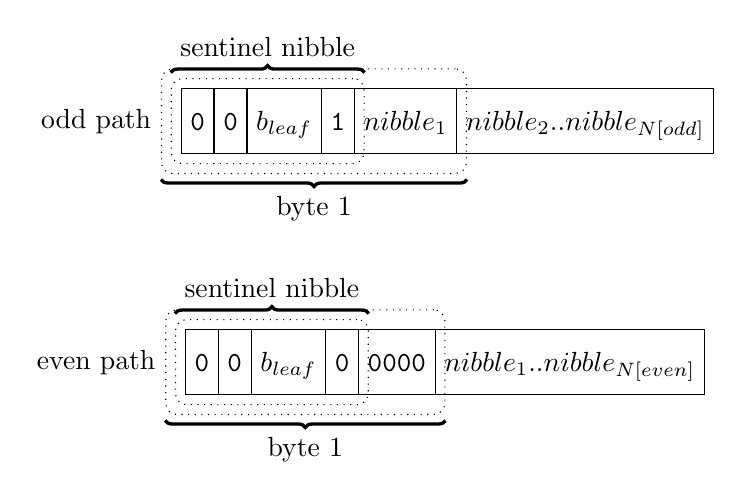
\begin{tikzpicture}[node distance=-\pgflinewidth]
			% odd tree node path
			\node[anchor=center] (lbl1) {odd path};
			\node[crecb,right=0.25cm of lbl1] (bit11) {\texttt{0}};
			\node[crecb,right=of bit11] (bit12) {\texttt{0}};
			\node[crecb,right=of bit12] (bit13) {$b_{leaf}$};
			\node[crecb,right=of bit13] (bit14) {\texttt{1}};

			\node[crecb,right=of bit14] (nibble12) {$nibble_1$};
			\node[crecb,right=of nibble12] {$nibble_2..nibble_{N [odd]}$};

			\node[fit=(bit11)(bit12)(bit13)(bit14), draw, dotted, rounded corners] (nibble11) {};
			\draw[decorate,decoration={brace,raise=2pt},very thick] (nibble11.north west) -- node[above=4pt] {sentinel nibble} (nibble11.north east);

			\node[fit=(nibble11)(nibble12), draw, dotted, rounded corners] (byte11) {};
			\draw[decorate,decoration={brace,mirror,raise=2pt},very thick] (byte11.south west) -- node[below=4pt] {byte 1} (byte11.south east);

			% even tree node path
			\node[anchor=center, below=2.5cm of lbl1] (lbl2) {even path};
			\node[crecb,right=0.25cm of lbl2] (bit21) {\texttt{0}};
			\node[crecb,right=of bit21] (bit22) {\texttt{0}};
			\node[crecb,right=of bit22] (bit23) {$b_{leaf}$};
			\node[crecb,right=of bit23] (bit24) {\texttt{0}};

			\node[crecb,right=of bit24] (nibble22) {\texttt{0000}};
			\node[crecb,right=of nibble22] {$nibble_1..nibble_{N [even]}$};

			\node[fit=(bit21)(bit22)(bit23)(bit24), draw, dotted, rounded corners] (nibble21) {};
			\draw[decorate,decoration={brace,raise=2pt},very thick] (nibble21.north west) -- node[above=4pt] {sentinel nibble} (nibble21.north east);

			\node[fit=(nibble21)(nibble22), draw, dotted, rounded corners] (byte21) {};
			\draw[decorate,decoration={brace,mirror,raise=2pt},very thick] (byte21.south west) -- node[below=4pt] {byte 1} (byte21.south east);
		\end{tikzpicture}
	}{Tree node path encoding}
\end{figure}

A \emph{leaf node}\index{node!leaf} is composed of the following two items:
\begin{enumerate}
	\item{TreeNodePath: Encoded tree node path (with leaf bit set).}
	\item{ValueHash: Hash of the value associated with the key ending at the leaf.}
\end{enumerate}

The hash of a leaf node can be calculated by hashing its component parts: $$\textit{H(Leaf)}=H(TreeNodePath, ValueHash)$$.

A \emph{branch node}\index{node!branch} is composed of the following items:
\begin{enumerate}
	\item{TreeNodePath: Encoded tree node path (with leaf bit unset).}
	\item{$LinkHash_{0...15}$: Hashes of children where the index is the next nibble part of the path.
	When no child is present at an index, a zero hash should be used instead.}
\end{enumerate}

The hash of a branch node can be calculated by hashing its component parts: $$\textit{H(Branch)}=H(TreeNodePath, LinkHash_0,..LinkHash_{15})$$.

Reconstructing the earlier example with hex keys yields a tree that illustrates a more accurate view of how a \codenamespace tree is constructed.
Notice that each branch node index composes a single nibble of the path.
This is depicted in \autoref{fig:trees:hexCompact}.

\begin{figure}[ht]
	\nemtreelabeled{
		\tikzstyle{level 1}=[sibling distance=20em]
		\tikzstyle{level 3}=[sibling distance=16em]
		\tikzstyle{level 4}=[sibling distance=8em]
		\node (6) [red] {\texttt{6}}
			child { node (646F) [red] {\texttt{6F}}
				child { node (646F0000) {\texttt{000} [verb]} }
				child { node (646F67) [red] {\texttt{7}}
					child { node (646F6700) {\texttt{0} [puppy]} }
					child { node (646F6765) [red] {\texttt{5} [mascot]} }
				}
			}
			child { node (686F7273) {\texttt{6F7273} [stallion] } };

		\begin{scope}[every node/.style = {draw=none}]
			\path (6) -- (646F) node [red, above, pos=0.5] {{\texttt{4}}};
			\path (6) -- (686F7273) node [above, pos=0.5] {\texttt{8}};
			\path (646F) -- (646F0000) node [above, pos=0.5] {\texttt{0}};
			\path (646F) -- (646F67) node [red, above, pos=0.5] {{\texttt{6}}};
			\path (646F67) -- (646F6700) node [above, pos=0.5] {\texttt{0}};
			\path (646F67) -- (646F6765) node [red, above, pos=0.5] {{\texttt{6}}};
		\end{scope}
	}{
		Realistic patricia tree with branch and leaf nodes and all optimizations.
		Path to $mascot$ [\texttt{646F6765}] is highlighted.
	}{hexCompact}
\end{figure}

\subsection{Merkle Patricia Tree Proofs}

A merkle proof for existence requires a single node from each level of the tree.
In order to prove the existence of $\{key = \texttt{646F6765}, value = H(mascot)\}$, a client must:
\begin{enumerate}
	\item{Calculate $H(mascot)$ (remember, all leaf values are hashes).}
	\item{Request all nodes on the path $\texttt{646F6765}$: $Node_{6}$, $Node_{646F}$, $Node_{646F67}$.}
	\item{Verify that $Node_{646F67}::Link[6]$ is equal to $H(Leaf(mascot))$.}
	\item{Calculate $H(Node_{646F67})$ and verify that $Node_{6467}::Link[6]$ is equal to $H(Node_{646F67})$.}
	\item{Calculate $H(Node_{6467})$ and verify that $Node_{6}::Link[4]$ is equal to $H(Node_{6467})$.}
	\item{Existence is proven if all calculated and actual hashes match.}
\end{enumerate}

A merkle proof for non-existence requires a single node from each level of the tree.
In order to prove the non-existence of $\{key = \texttt{646F6764}, value = H(mascot)\}$, a client must:
\begin{enumerate}
	\item{Calculate $H(mascot)$ (remember, all leaf values are hashes).}
	\item{Request all nodes on the path $\texttt{646F6764}$: $Node_{6}$, $Node_{646F}$, $Node_{646F67}$.}
	\item{
		Verify that $Node_{646F67}::Link[5]$ is equal to $H(Leaf(mascot))$.
		Since $Link[5]$ is unset, this check will fail.
		If the value being searched for was in the tree, it must be linked to this node because of the determinism of the tree.
	 }
\end{enumerate}

	\section{Accounts and Addresses}
\label{sec:accounts}

\nemquote{
}{}

\codenamechapterfirstword uses elliptic curve cryptography to ensure confidentiality, authenticity and non-repudiability of all transactions.
Each account is a private+public Ed25519 keypair \nemrefparens{sec:cryptography} and is associated with a mutable state that is updated when transactions are accepted by the network.
Accounts are identified by addresses, which are derived in part from one way mutations of public keys.

\subsection{Addresses}

An \nind{address} is a base32\footnote{ \url{http://en.wikipedia.org/wiki/Base32} } encoded triplet consisting of:
\begin{itemize}
	\item{network byte}
	\item{160-bit hash of the account's public key}
	\item{4 byte checksum}
\end{itemize}

The checksum allows for quick recognition of mistyped addresses.
It is possible to send mosaics to any valid address even if the address has not previously participated in any transaction.
If nobody owns the private key of the account to which the mosaics are sent, the mosaics are most likely lost forever.

\subsection{Address Derivation}
In order to convert a public key to an address, the following steps are performed:
\begin{enumerate}
	\item{Perform 256-bit SHA3 on the public key}
	\item{Perform 160-bit RIPEMD of hash resulting from step 1}
	\item{Prepend network version byte to RIPEMD hash}
	\item{Perform 256-bit SHA3 on the result, take the first four bytes as a checksum}
	\item{Concatenate output of step 3 and the checksum from step 4}
	\item{Encode result using base32}
\end{enumerate}

\begin{figure}
	\nemcenterwithcaption{
		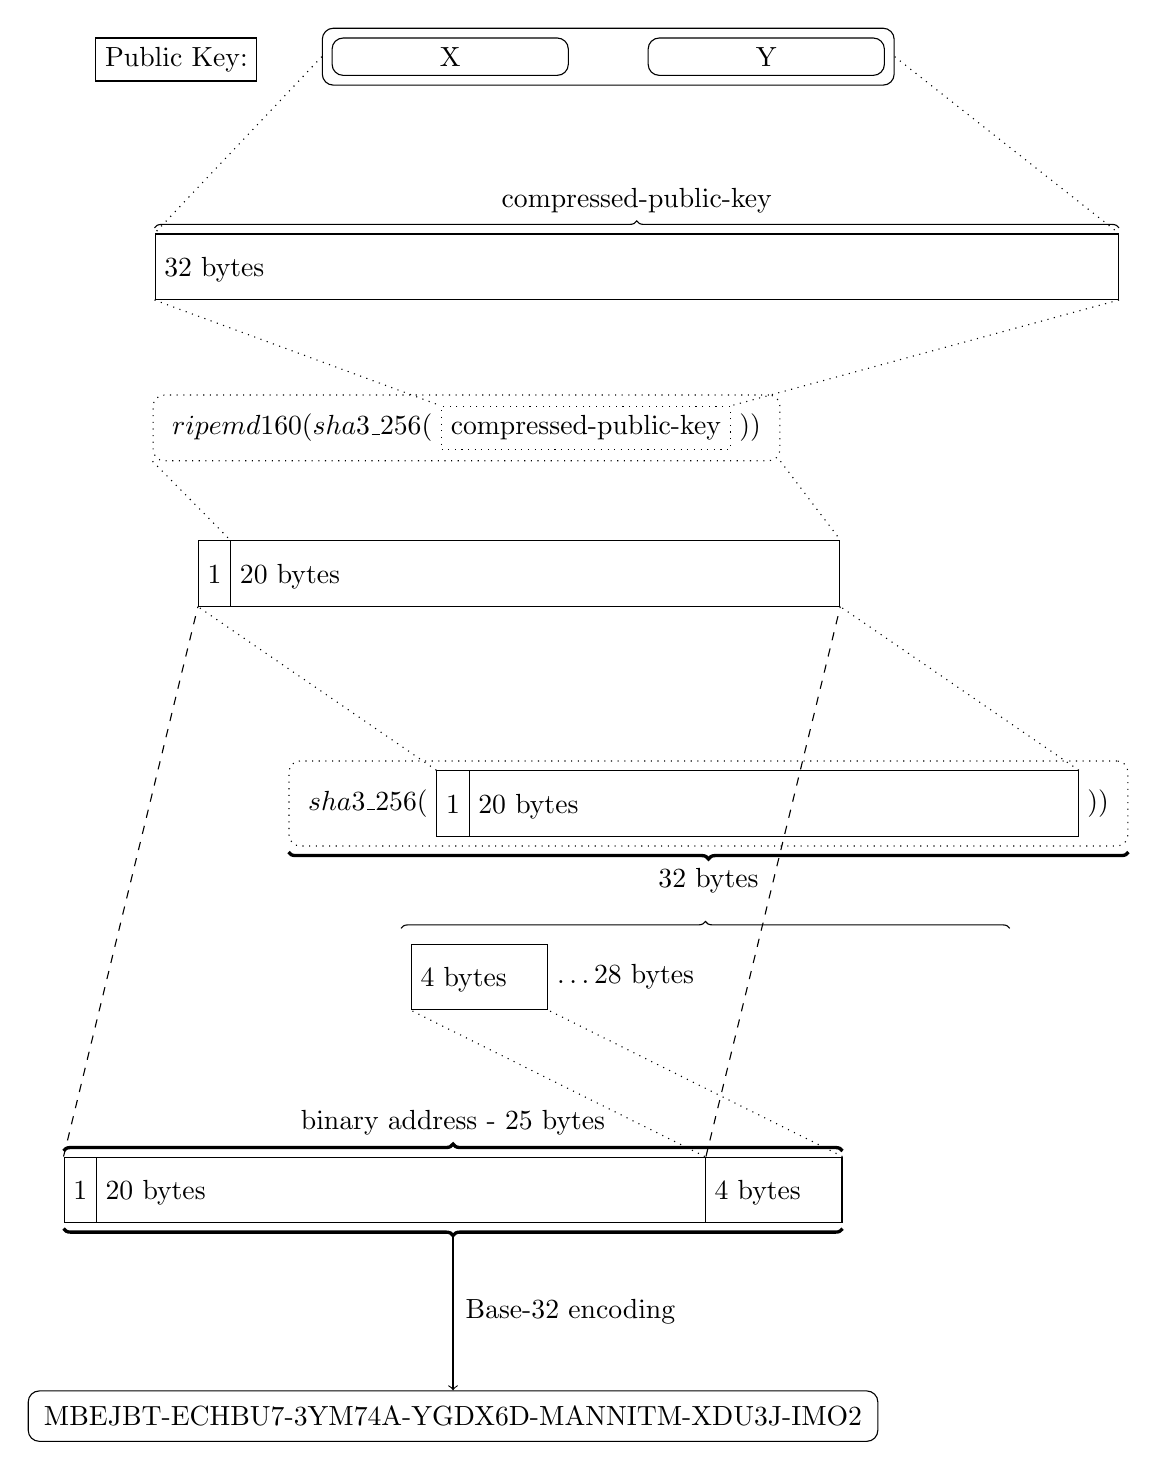
\begin{tikzpicture}[node distance=-\pgflinewidth]

	% First row, public key
	\node[draw,anchor=north west] (pubkeyLabel) at (0,0) {Public Key: };

	\node[crou,anchor=north west,minimum width=3cm] (pkx) at (3, 0) {X};
	\node[crou,minimum width=3cm, right=1cm of pkx] (pky) {Y};

	\node[fit=(pkx)(pky),crou] (xy) {};

	% join lines
	\node[crecb,below left=2cm and -10cm of pkx,text width=12cm] (bpk32) {32 bytes};

	% second row
	\draw[decorate,decoration={brace,raise=2pt}] (bpk32.north west) --
		node[above=4pt] (bpkLabel) {compressed-public-key}
		(bpk32.north east);

	\draw[dotted] (xy.west) -- (bpk32.north west);
	\draw[dotted] (xy.east) -- (bpk32.north east);

	% invisible
	\node[fit=(bpk32)(bpkLabel)] (bpk) {};


	% third row - ripeMD

	% it's easier to do it this way, as problems with paths show up when using nested tikzpicture
	\node[below left=1.5cm and -2cm of bpk,anchor=center] (ripeInner) { $\mathfunc{ripemd160}(\mathfunc{sha3\_256}($ };
	\node[right=of ripeInner, draw, dotted,rounded corners=0] (bpkInnerLabel) {compressed-public-key};
	\node[right=of bpkInnerLabel] (ripeInner2) { $)) $ };

	\node[fit=(ripeInner)(bpkInnerLabel)(ripeInner2), draw, dotted, rounded corners] (ripe) {};

	\draw[dotted] (bpk32.south west) -- (bpkInnerLabel.north west);
	\draw[dotted] (bpk32.south east) -- (bpkInnerLabel.north east);


	% Fourth row - network byte + ripemd output
	\node[crecb,below left=1cm and -1cm of ripe] (brmd1) {1};
	\node[crecb,right=of brmd1,text width=7.5cm] (brmd20) {20 bytes};

	\draw[dotted] (ripe.south west) -- (brmd20.north west);
	\draw[dotted] (ripe.south east) -- (brmd20.north east);

	% Fifth row - SHA3(version + ripe)
	\node[below right=2.5cm and -6cm of brmd20,anchor=center] (checkInner) { $\mathfunc{sha3\_256(}$ };
	\node[crecb,right=of checkInner] (bInnerRmd1) {1};
	\node[crecb,right=of bInnerRmd1,text width=7.5cm] (bInnerRmd20) {20 bytes};
	\node[right=of bInnerRmd20] (checkInner2) { $)) $ };

	\draw[dotted] (bInnerRmd1.north west) -- (brmd1.south west);
	\draw[dotted] (bInnerRmd20.north east) -- (brmd20.south east);

	\node[fit=(checkInner)(bInnerRmd1)(bInnerRmd20)(checkInner2), draw, dotted, rounded corners] (check) {};

	\draw[decorate,decoration={brace,mirror,raise=2pt},very thick] (check.south west) -- node[below=4pt] (check32) {32 bytes} (check.south east);


	% Sixth row - sha3 output
	\node[below=1.5cm of bInnerRmd20,text width=5.5cm] (check28) {\ldots 28 bytes};
	\node[crecb,left=of check28,text width=1.5cm] (check4) {4 bytes};
	\node[fit=(check4)(check28)] (checkGroup) {};
	\draw[decorate,decoration={brace,raise=2pt}] (checkGroup.north west) -- (checkGroup.north east);

	% Seventh row - binary address
	\node[crecb,below=2cm of check28,text width=1.5cm] (bAddr4) {4 bytes};
	\node[crecb,left=of bAddr4,text width=7.5cm] (bAddr20) {20 bytes};
	\node[crecb,left=of bAddr20] (bAddr1) {1};
	\node[fit=(bAddr1)(bAddr20)(bAddr4)] (binaryAddress) {};

	\draw[decorate,decoration={brace,raise=2pt},very thick] (bAddr1.north west) -- node[above=4pt] {binary address - 25 bytes} (bAddr4.north east);
	\draw[decorate,decoration={brace,mirror,raise=2pt},very thick] (bAddr1.south west) -- node[below=4pt] (binAddr) {} (bAddr4.south east);


	% final association
	\draw[dotted] (bAddr4.north west) -- (check4.south west);
	\draw[dotted] (bAddr4.north east) -- (check4.south east);

	\draw[dashed,thin] (bAddr1.north west) -- (brmd1.south west);
	\draw[dashed,thin] (bAddr20.north east) -- (brmd20.south east);

	\node[draw,below=2cm of binaryAddress,rounded corners,solid,inner sep=0.2cm] (nanemo) {
		MBEJBT-ECHBU7-3YM74A-YGDX6D-MANNITM-XDU3J-IMO2};
	\draw[solid,thin,->] (binaryAddress.south) -- node[right=1pt] {Base-32 encoding} (nanemo.north);

\end{tikzpicture}

	}{Address generation}
\end{figure}

\pagebreak

\subsection{Address Aliases}
\index{alias address}
An address can have one or more aliases assigned using an address alias transaction\footnote{
See \url{https://nemtech.github.io/concepts/namespace.html\#address-alias-transaction}}.
All transactions accepting addresses support using either a public key derived address or an address alias.
In case of such transactions, the format of the address alias field is:
\begin{itemize}
	\item{network byte ORed with value 1}
	\item{8 byte namespace id that is an alias}
	\item{16 zero bytes}
\end{itemize}

\subsection{Intentional Address Collision}
It is possible that two different public keys will yield the same address.
If such an address contains any valuable assets \textbf{AND} has not been associated with a public key earlier (for example, by sending a transaction from the account), it would be possible for an attacker to withdraw funds from such an account.

In order for the attack to succeed, the attacker would need to find a private+public keypair such that the SHA3\_256 of the public key would \textbf{at the same time} be equal to the ripemd-160 preimage of the 160-bit hash mentioned above.
Since SHA3\_256 offers 128 bits of security, it is mathematically improbable for a single SHA3\_256 collision to be found.
Due to similarities between \codenamespace addresses and Bitcoin addresses, the probability of causing a \codenamespace address collision is roughly the same as that of causing a Bitcoin address collision.

	\section{Transactions}
\label{sec:transactions}

\nemquote{
}{}

\nemchapterfirstletter{T}{ransactions} are instructions that modify the global chain state.
They are processed atomically and grouped into blocks.
If any part of a transaction fails processing, the global chain state is reset to the state prior to the transaction application attempt.

There are two fundamental types of transactions: basic transactions and aggregate transactions.
Basic transactions represent a single operation and require a single signature.
Aggregate transactions are containers of one or more transactions that may require multiple signatures.

Aggregate transactions allow basic transactions to be combined into potentially complex operations and executed atomically.
This increases developer flexibility relative to a system that only guarantees atomicity for individual operations while still constraining the global set of operations allowed to a finite set.
It does not require the introduction of a Turing-complete language and all of its inherent disadvantages.

\subsection{Basic Transaction}

A basic transaction is composed of both cryptographically verifiable and unverifiable data.
All verifiable data is contiguous and is signed by the transaction signer.
All unverifiable data is either ignored (e.g. padding bytes) or deterministically computable from verifiable data.
Each basic transaction requires verification of exactly one signature.

None of the unverifiable header fields need to be verified.
\texttt{Size} is the serialized size of the transaction and can always be derived from verifiable transaction data.
\texttt{Signature} is an output from signing and an input to verification.
\texttt{SignerPublicKey} is an input to both signing and verification.
In order for a transaction to pass signature verification, both \texttt{Signature} and \texttt{SignerPublicKey} must be matched with the verifiable data, which has a length relative to \texttt{Size}.
$$verify(T::Signature, T::SignerPublicKey, VerifiableDataBuffer(T))$$

\texttt{Reserved} bytes are used for padding transactions so that all integral fields and cryptographic primitives have natural alignment.
Since these bytes are meaningless, they can be stripped without invalidating any cryptographic guarantees.

Binary layouts for all transaction types are specified in catapult's open source schema language
\footnote{Schemas can be found at https://github.com/nemtech/catbuffer}.
Please refer to the published schemas for the most up to date specifications.

\begin{figure}[H]
	\nemcenterwithcaption{
		\begin{subfigure}{.5\textwidth}
			\nemmemorylayout{
				\begin{leftwordgroup}{\texttt{0x00}}
					\bitbox{4}{Size} \bitbox{4}{Reserved}
				\end{leftwordgroup} \\
				\nemmemorymultiwordbox{\texttt{0x08}}{Signature}{7} \\
				\nemmemorymultiwordbox{\texttt{0x48}}{SignerPublicKey}{3} \\
				\begin{leftwordgroup}{\texttt{0x68}}
					\bitbox{4}{Reserved} \bitbox[]{4}{}
				\end{leftwordgroup}
			}{Header (unsigned)}
		\end{subfigure}%
		\begin{subfigure}{.5\textwidth}
			\nemmemorylayout{
				\begin{leftwordgroup}{\texttt{0x6C}}
					\bitbox[br]{4}{} \bitbox{4}{V, N, T}
				\end{leftwordgroup} \\
				\begin{leftwordgroup}{\texttt{0x70}}
					\wordbox[tlr]{1}{MaxFee}
				\end{leftwordgroup} \\
				\begin{leftwordgroup}{\texttt{0x78}}
					\wordbox{1}{Deadline}
				\end{leftwordgroup} \\
				\nemmemorymultiwordboxskipped{\texttt{0x80}}{Payload}{} \\
			}{Verifiable data}
		\end{subfigure}
	}{Basic transaction binary layout}
\end{figure}

\subsection{Aggregate Transaction}

The layout of an aggregate transaction is more complex than that of a basic transaction, but there are some similarities.
An aggregate transaction shares the same unverifiable header as a basic transaction, and this data is processed in the same way.
Additionally, an aggregate transaction has a footer of unverifiable data followed by embedded transactions and cosignatures.

An aggregate transaction can always be submitted to the network with all requisite cosignatures.
In this case, it is said to be \emph{complete} and it is treated like any other transaction without any special processing.

API nodes can also accept \emph{bonded} aggregate transactions that have incomplete cosignatures.
The submitter must pay a bond that is returned if and only if all requisite cosignatures are collected before the transaction times out.
Assuming this bond is paid upfront, an API node will collect cosignatures associated with this transaction until it either has sufficient signatures or times out.

\texttt{TransactionsHash} is the most important field in an aggregate transaction.
It is the merkle root hash of the hashes of the embedded transactions stored within the aggregate.
In order to compute this field, a merkle tree is constructed by adding each embedded transaction hash in natural order.
The resulting root hash is assigned to this field.

None of the unverifiable footer fields need to be verified.
\texttt{PayloadSize} is a computed size field that must be correct in order to extract the exact same embedded transactions that were used to calculate \texttt{TransactionsHash}.
\texttt{Reserved} bytes, again, are used for padding and have no intrinsic meaning.

\begin{figure}[H]
	\nemcenterwithcaption{
		\begin{subfigure}{.33\textwidth}
			\nemmemorylayout{
				\begin{leftwordgroup}{\texttt{0x00}}
					\bitbox{4}{Size} \bitbox{4}{Reserved}
				\end{leftwordgroup} \\
				\nemmemorymultiwordbox{\texttt{0x08}}{Signature}{7} \\
				\nemmemorymultiwordbox{\texttt{0x48}}{SignerPublicKey}{3} \\
				\begin{leftwordgroup}{\texttt{0x68}}
					\bitbox{4}{Reserved} \bitbox[]{4}{}
				\end{leftwordgroup}
			}{Header (unsigned)}
		\end{subfigure}%
		\begin{subfigure}{.33\textwidth}
			\nemmemorylayout{
				\begin{leftwordgroup}{\texttt{0x6C}}
					\bitbox[br]{4}{} \bitbox{4}{V, N, T}
				\end{leftwordgroup} \\
				\begin{leftwordgroup}{\texttt{0x70}}
					\wordbox[tlr]{1}{MaxFee}
				\end{leftwordgroup} \\
				\begin{leftwordgroup}{\texttt{0x78}}
					\wordbox{1}{Deadline}
				\end{leftwordgroup} \\
				\begin{leftwordgroup}{\texttt{0x80}}
					\wordbox{1}{TransactionsHash}
				\end{leftwordgroup}
			}{Verifiable data}
		\end{subfigure}%
		\begin{subfigure}{.33\textwidth}
			\nemmemorylayout{
				\begin{leftwordgroup}{\texttt{0x88}}
					\bitbox{4}{\tiny PayloadSize} \bitbox{4}{Reserved}
				\end{leftwordgroup} \\
				\nemmemorymultiwordboxskipped{\texttt{0x90}}{Embedded}{Transactions} \\
				\nemmemorymultiwordboxskipped{}{Cosignatures}{}
			}{Unverifiable footer}
		\end{subfigure}
	}{Aggregate transaction header binary layout}
\end{figure}

\subsubsection{Embedded Transaction}

An embedded transaction is a transaction that is contained within an aggregate transaction.
Compared to a basic transaction, the header is smaller, but the transaction-specific data is the same.
\texttt{Signature} is removed because all signature information is contained in cosignatures.
\texttt{MaxFee} and \texttt{Deadline} are removed because they are specified by the parent aggregate transaction.

Client implementations can use the same code to construct the custom parts of either a basic or embedded transaction.
The only difference is in the creation and application of different headers.

Not all transactions are supported as embedded transactions.
For example, an aggregate transaction cannot be embedded within another aggregate transaction.

\begin{figure}[H]
	\nemcenterwithcaption{
		\begin{subfigure}{.5\textwidth}
			\nemmemorylayout{
				\begin{leftwordgroup}{\texttt{0x00}}
					\bitbox{4}{Size} \bitbox{4}{Reserved}
				\end{leftwordgroup} \\
				\nemmemorymultiwordbox{\texttt{0x08}}{SignerPublicKey}{3} \\
				\begin{leftwordgroup}{\texttt{0x28}}
					\bitbox{4}{Reserved} \bitbox[]{4}{}
				\end{leftwordgroup}
			}{Header (unsigned)}
		\end{subfigure}%
		\begin{subfigure}{.5\textwidth}
			\nemmemorylayout{
				\begin{leftwordgroup}{\texttt{0x2C}}
					\bitbox[br]{4}{} \bitbox{4}{V, N, T}
				\end{leftwordgroup} \\
				\nemmemorymultiwordboxskipped{\texttt{0x30}}{Payload}{}
			}{Verifiable data}
		\end{subfigure}
	}{Embedded transaction binary layout}
\end{figure}

\subsubsection{Cosignature}

A cosignature is a pair composed of a public key and its corresponding signature.
Zero or more cosignatures are appended at the end of an aggregate transaction.
Cosignatures are used to cryptographically verify an aggregate transaction involving multiple parties.

\begin{figure}[H]
	\nemcenter{
		\nemmemorylayout{
			\nemmemorymultiwordbox{\texttt{0x00}}{SignerPublicKey}{3} \\
			\nemmemorymultiwordbox{\texttt{0x20}}{Signature}{7}
		}{Cosignature binary layout}
	}{}
\end{figure}

In order for an aggregate transaction \texttt{A} to pass verification, it must pass basic transaction signature verification and have a cosignature for every embedded transaction signer
\footnote{In the case of multisignature accounts, there must be enough cosignatures to satisfy the multisignature account constraints.}.

Like any transaction, an aggregate transaction, must pass basic transaction signature verification.
$$verify(A::Signature, A::SignerPublicKey, VerifiableDataBuffer(A))$$

Additionally, all cosignatures must pass signature verification.
Notice that cosigners sign the hash of an aggregate transaction data, not the data directly.
$$\sum_{0\leq i \leq N_C} verify(C::Signature, C::SignerPublicKey, H(VerifiableDataBuffer(A)))$$

Finally, there must be a cosignature that corresponds to and satisfies each embedded transaction signer.

\subsubsection{Extended Layout}

The aggregate transaction layout described earlier was correct with one simplification.
All embedded transactions are padded so that they end on 8-byte boundaries.
This ensures that all embedded transactions and cosignatures begin on 8-byte boundaries as well.
The padding bytes are never signed nor included in any hashes.

\begin{figure}[H]
	\nemcenter{
		\nemmemorylayout{
			\begin{leftwordgroup}{}
				\bitbox{4}{\tiny PayloadSize} \bitbox{4}{Reserved}
			\end{leftwordgroup} \\
			\nemmemorymultiwordboxskipped{}{Embedded}{Transaction 1} \\
			\begin{leftwordgroup}{}
				\wordbox{1}{\emph{optional} padding}
			\end{leftwordgroup} \\
			\nemmemorymultiwordboxskipped{}{Embedded}{Transaction 2} \\
			\begin{leftwordgroup}{}
				\wordbox{1}{\emph{optional} padding}
			\end{leftwordgroup} \\
			\nemmemorymultiwordboxskipped{}{Cosignatures}{}
		}{Aggregate transaction footer with padding}
	}
\end{figure}

	\section{Blocks}
\label{sec:blocks}

\nemquote{
}{}

\codenamechapterfirstword is, at its core, a blockchain.
A blockchain is an ordered collection of blocks.
Understanding the parts of a \codenamespace block is fundamental to understanding the platform's capabilities.

The layout of a block is similar to the layout of an aggregate transaction (\nemref{sec:transactions:aggregate}).
A block shares the same unverifiable header as an aggregate transaction, and this data is processed in the same way.
Likewise, a block has a footer of unverifiable data followed by transactions.
Unlike an aggregate transaction, a block is followed by basic - not embedded - transactions, and each transaction within a block is signed independently of the block signer\footnote{
In an aggregate transaction, the account creating the aggregate transaction must sign the transaction's data in order for it to be valid.
In a block, the block signer does not need to sign the data of any transaction contained within it.
}.
This allows any transaction satisfying all conditions to be included in any block.

None of the unverifiable footer fields need to be verified.
\texttt{Reserved} bytes are used for padding and have no intrinsic meaning.

\begin{figure}
	\nemcenterwithcaption{
		\begin{subfigure}{.33\textwidth}
			\nemmemorylayout{
				\begin{leftwordgroup}{\texttt{0x00}}
					\bitbox{4}{Size} \bitbox{4}{Reserved}
				\end{leftwordgroup} \\
				\nemmemorymultiwordbox{0x08}{Signature}{7} \\
				\nemmemorymultiwordbox{0x48}{SignerPublicKey}{3} \\
				\begin{leftwordgroup}{\texttt{0x68}}
					\bitbox{4}{Reserved} \bitbox[]{4}{}
				\end{leftwordgroup}
			}{Header (unsigned)}
		\end{subfigure}%
		\begin{subfigure}{.33\textwidth}
			\nemmemorylayout{
				\begin{leftwordgroup}{\texttt{0x6C}}
					\bitbox[br]{4}{} \bitbox{4}{V, N, T}
				\end{leftwordgroup} \\
				\begin{leftwordgroup}{\texttt{0x70}}
					\wordbox{1}{Height}
				\end{leftwordgroup} \\
				\begin{leftwordgroup}{\texttt{0x78}}
					\wordbox{1}{Timestamp}
				\end{leftwordgroup} \\
				\begin{leftwordgroup}{\texttt{0x80}}
					\wordbox{1}{Difficulty}
				\end{leftwordgroup} \\
				\nemmemorymultiwordbox{0x88}{PreviousBlockHash}{3} \\
				\nemmemorymultiwordbox{0xA8}{TransactionsHash}{3} \\
				\nemmemorymultiwordbox{0xC8}{ReceiptsHash}{3} \\
				\nemmemorymultiwordbox{0xE8}{StateHash}{3} \\
				\nemmemorymultiwordbox{0x108}{\small BeneficiaryPublicKey}{3} \\
				\begin{leftwordgroup}{\texttt{0x128}}
					\bitbox{4}{\tiny FeeMultiplier} \bitbox[]{4}{}
				\end{leftwordgroup}
			}{Verifiable data}
		\end{subfigure}%
		\begin{subfigure}{.33\textwidth}
			\nemmemorylayout{
				\begin{leftwordgroup}{\texttt{0x12C}}
					\bitbox[br]{4}{} \bitbox{4}{Reserved}
				\end{leftwordgroup} \\
				\nemmemorymultiwordboxskipped{0x130}{Transactions}{}
			}{Unverifiable footer}
		\end{subfigure}
	}{Block header binary layout}
\end{figure}

\subsection{Block Fields}

\field{Height} is the block sequence number.
The first block, called the \nind{nemesis block}, has a height of one.
Each successive block increments the height of the previous block by one.

\field{Timestamp} is the number of milliseconds that have elapsed since the nemesis block.
Each successive block must have a timestamp greater than that of the previous blocks because block time is strictly increasing.
Each network tries to keep the average time between blocks close to \textit{target block time}.

\field{Difficulty} is described in detail in \nemref{sec:blockchain:difficulty}.

\field{PreviousBlockHash} is the hash of the previous block.
This is used to guarantee that all blocks within a blockchain are linked and deterministically ordered.

\field{TransactionsHash} is the merkle root hash of the hashes of the transactions stored within the block
\footnote{This field has the same purpose as the identically named field in an aggregate transaction.}.
In order to compute this field, a merkle tree is constructed by adding each transaction hash in natural order.
The resulting root hash is assigned to this field.

\field{ReceiptsHash} is the merkle root hash of the hashes of the receipts produced while processing the block.
When a network is configured without \nemsetting{network}{enableVerifiableReceipts}, this field must be zeroed in all blocks.
See \nemref{sec:blocks:receipts}.

\field{StateHash} is the hash of the global blockchain state after processing the block.
When a network is configured without \nemsetting{network}{enableVerifiableState}, this field must be zeroed in all blocks.
Otherwise, it's calculated as described in \nemref{sec:blocks:statehash}.

\field{BeneficiaryPublicKey} is the account that will be allocated the block's beneficiary share when the network has a nonzero \nemsetting{network}{harvestBeneficiaryPercentage}.
This field can be set to any account, even one that isn't yet known to the network.
This field is set by the node owner when a new block is harvested.
If this account is set to one owned by the node owner, the node owner will share in fees paid in all blocks harvested on its node.
This, in turn, incentivizes the node owner to run a strong node with many delegated harvesters.

\field{FeeMultiplier} is a multiplier that is used to calculate the effective fee of each transaction contained within a block.
The \nemsetting{node}{minFeeMultiplier} is set by the node owner and can be used to accomplish varying goals, including maximization of profits or confirmed transactions.
Assuming a block $B$ containing a transaction $T$, the effective transaction fee can be calculated as:
$$\mathfunc{effectiveFee}(T) = \structField{B}{FeeMultiplier} \cdot \mathfunc{sizeof}(T)$$
If the effective fee is greater than the transaction \field{MaxFee}, the transaction signer keeps the difference.
Only the effective fee is deducted from the transaction signer and credited to the harvester.
Further information about fee multipliers can be found in\nemref{sec:blockchain:generation}.

\subsection{Receipts}
\label{sec:blocks:receipts}

During the execution of a block, zero or more receipts are generated.
Receipts are primarily used to communicate state changes triggered by side effects to clients.
In this way, they allow simpler clients to still be aware of complex state changes.

For example, a namespace expiration is triggered by the number of blocks that have been confirmed since the namespace was created.
While the triggering event is in the blockchain, there is no indication of this state change in the block at which the expiration occurs.
Without receipts, a client would need to keep track of all namespaces and expiration heights.
With receipts, a client merely needs to monitor for expiration receipts.

Another example is around harvest rewards.
Receipts are produced that indicate the main - not delegated - account that gets credited and any beneficiary splits.
They also communicate the amount of currency created by inflation.

Receipts are grouped into three different types of statements and collated by receipt sources.
The three types of statements are transaction, address resolution and mosaic resolution.

\subsubsection{Receipt Source}

Each part of a block that is processed is assigned a two-part block-scoped identifier.
The source (0, 0) is always used to identify block-triggered events irrespective of the number of transactions in a block.

\begin{table}[ht]
	\nemcenterwithcaption{
		\begin{tabular}{|p{0.20\linewidth}|p{0.40\linewidth}|p{0.40\linewidth}|}
			\hline
			Source & Primary Id & Secondary Id \\
			\hline
			Block & 0 & 0 \\
			Transaction & 1-based index within the block & 0 \\
			Embedded Transaction & 1-based index of containing aggregate within the block & 1-based index within the aggregate \\
			\hline
		\end{tabular}
	}{Receipt source values}
\end{table}

\subsubsection{Transaction Statement}

Transaction statements are used to group receipts that have a shared receipt source.
Each statement is composed of a receipt source and one or more receipts.
Accordingly, each receipt source that generates a receipt will have exactly one corresponding transaction statement.

\begin{figure}[H]
	\nemcenterwithcaption{
		\begin{subfigure}{.5\textwidth}
			\nemmemorylayout{
				\begin{leftwordgroup}{\texttt{0x00}}
					\bitbox{4}{Size} \bitbox{2}{V} \bitbox{2}{T}
				\end{leftwordgroup} \\
				\begin{leftwordgroup}{\texttt{0x08}}
					\wordbox{1}{ReceiptSource}
				\end{leftwordgroup} \\
				\nemmemorymultiwordboxskipped{0x10}{Receipts}{} \\
			}{Transaction statement binary layout}
		\end{subfigure}%
		\begin{subfigure}{.5\textwidth}
			\nemmemorylayout{
				\begin{leftwordgroup}{\texttt{0x00}}
					\bitbox{4}{Size} \bitbox{2}{V} \bitbox{2}{T}
				\end{leftwordgroup} \\
				\nemmemorymultiwordboxskipped{0x08}{Payload}{}
			}{Receipt binary layout}
		\end{subfigure}
	}{Transaction statement layout}
\end{figure}

Transaction statement data is not padded because it is only written during processing and never read, so padding yields no server performance benefit.
A transaction statement hash is constructed by concatenating and hashing all statement data excepting \field{Size} fields, which are derivable from other data.

\subsubsection{Resolution Statements}

Resolution statements are used exclusively for indicating alias resolutions.
They allow a client to always resolve an unresolved value even when it changes within a block.
Theoretically, two unresolved aliases within the same block could resolve to different values if there is an alias change between their usages.
Each statement is composed of an unresolved value and one or more resolutions in order to support this.

There are two types of resolution statements - address and mosaic - corresponding to the two types of aliases.
Although \autoref{fig:blocks:mosaicResolutionStatementLayout} illustrates the layout of a mosaic resolution statement, the layout of an address resolution statement is nearly identical.
The only difference is that the resolved and unresolved values are 25-byte addresses instead of 8-byte mosaic ids.

\begin{figure}[H]
	\nemcenterwithcaption{
		\begin{subfigure}{.5\textwidth}
			\nemmemorylayout{
				\begin{leftwordgroup}{\texttt{0x00}}
					\bitbox{4}{Size} \bitbox{2}{V} \bitbox{2}{T}
				\end{leftwordgroup} \\
				\begin{leftwordgroup}{\texttt{0x08}}
					\wordbox{1}{\small MosaicId Unresolved}
				\end{leftwordgroup} \\
				\nemmemorymultiwordboxskipped{0x10}{Resolution}{Entries} \\
			}{Mosaic resolution statement binary layout}
		\end{subfigure}%
		\begin{subfigure}{.5\textwidth}
			\nemmemorylayout{
				\begin{leftwordgroup}{\texttt{0x00}}
					\bitbox{8}{ReceiptSource}
				\end{leftwordgroup} \\
				\begin{leftwordgroup}{\texttt{0x08}}
					\bitbox{8}{\small MosaicId Resolved}
				\end{leftwordgroup} \\
			}{Resolution entry binary layout}
		\end{subfigure}
	}{Mosaic resolution statement layout\label{fig:blocks:mosaicResolutionStatementLayout}}
\end{figure}

Resolution statement data is not padded because it is only written during processing and never read, so padding yields no server performance benefit.
A resolution statement hash is constructed by concatenating and hashing all statement data excepting \field{Size} fields, which are derivable from other data.

It is important to note that a resolution statement is only produced when a resolution occurs.
If an alias is registered or changed in a block, but not used in that block, no resolution statement will be produced.
However, a resolution statement will be produced by each block that contains that alias and requires it to be resolved.

\subsubsection{Receipt Hash}

In order to calculate a block's receipt hash, first all statements generated during block processing are collected.
Then a merkle tree is created by adding all statement hashes in the following order:

\begin{enumerate}
\item{Hashes of transaction statements ordered by receipt source.}
\item{Hashes of address resolution statements ordered by unresolved address.}
\item{Hashes of mosaic resolution statements ordered by unresolved mosaic id.}
\end{enumerate}

When a network is configured with \nemsetting{network}{enableVerifiableReceipts}, the root hash of this merkle tree is set as the block's \field{ReceiptHash}.
A client can perform a merkle proof to prove a particular statement was produced during the processing of a specific block.

\subsection{State Hash}
\label{sec:blocks:statehash}

\codenamespace stores the global blockchain state across multiple typed state repositories.
For example, the account state is stored in one repository and the multsignature state is stored in another.
Each repository is a simple key value store.
The specific repositories present in a network are determined by the transaction plugins enabled by that network.

When a network is configured with \nemsetting{network}{enableVerifiableState}, a patricia tree is created for each repository.
This produces a single hash that deterministically fingerprints each repository.
Accordingly, assuming $N$ repositories, $N$ hashes deterministically fingerprint the global blockchain state.

It is possible to store all $N$ hashes directly in each block header, but this is undesirable.
Each block header should be as small as possible because all clients, minimally, need to sync all headers to verify a chain is rooted to the nemesis block.
Additionally, adding or removing functionality could change the number of repositories ($N$) and the format of the block header.

Instead, all root hashes are concatenated\footnote{The concatenation order is fixed and determined by the repository id.} and hashed to calculate the \field{StateHash},
which is a single hash that deterministically fingerprints the global blockchain state.
\begin{align*}
\mathit{RepositoryHashes} = \: & 0 \\
\mathit{RepositoryHashes} = \: & \sum_{0\leq i \leq N} \mathfunc{concat}(\mathit{RepositoryHashes}, \mathit{RepositoryHash}_i) \\
\mathit{StateHash} = \: & H(\mathit{RepositoryHashes})
\end{align*}

\subsection{Extended Layout}

The block layout described earlier was correct with one simplification\footnote{
This is consistent with the extended layout of an aggregate transaction as well.}.
All transactions are padded so that they end on 8-byte boundaries.
This ensures that all transactions begin on 8-byte boundaries as well.
The padding bytes are never signed nor included in any hashes.

\begin{figure}[H]
	\nemcenter{
		\nemmemorylayout{
			\begin{leftwordgroup}{}
				\bitbox[br]{4}{} \bitbox{4}{Reserved}
			\end{leftwordgroup} \\
			\nemmemorymultiwordboxskipped{}{Transaction 1}{} \\
			\begin{leftwordgroup}{}
				\wordbox{1}{\emph{optional} padding}
			\end{leftwordgroup} \\
			\nemmemorymultiwordboxskipped{}{Transaction 2}{} \\
			\begin{leftwordgroup}{}
				\wordbox{1}{\emph{optional} padding}
			\end{leftwordgroup}
		}{Block transaction footer with padding}
	}
\end{figure}

	\section{Blockchain}
\label{sec:blockchain}

\nemquote{
}{}

\codenamespace is centered around a public ledger called the blockchain that links blocks together.
The complete transaction history is held in the blockchain.
All blocks, and transactions within blocks, are deterministically and cryptographically ordered.
The maximum number of transactions per block can be configured per-network.

\subsection{Block Difficulty}
\index{block!difficulty}
\label{sec:blockchain:difficulty}

The nemesis block has a predefined \nind{initial difficulty} of $10^{14}$.
All difficulties are clamped between a minimum of $10^{13}$ and a maximum of $10^{15}$.

The difficulty for a new block is derived from the difficulties and timestamps of the most recently confirmed blocks.
The number of blocks taken into consideration is configurable per-network.

If less than \nemsetting{network}{maxDifficultyBlocks} are available, only those available are taken into account.
Otherwise, the difficulty is calculated from the last $n$ blocks in the following way:
\begin{align*}
\tag{average difficulty} d &= \frac{1}{n}\sum_{i=1}^n (\text{difficulty of $block_i$}) \\
\tag{average creation time} t &= \frac{1}{n}\sum_{i=1}^n (\text{time to create $block_i$}) \\
\tag{new difficulty} \mathit{difficulty} &= d \; \frac{\nemsetting{network}{blockGenerationTargetTime}}{t}
\end{align*}

This algorithm produces blocks with an average time close to the desired \nemsetting{network}{blockGenerationTargetTime} network setting.

If the new difficulty is more than 5\% larger or smaller than the difficulty of the last block, then the change is capped to 5\%.
The maximum change rate of 5\% per block makes it hard for an attacker with considerably less than 50\% importance to create a better chain in secret.
Block times will be considerably higher than \nemsetting{network}{blockGenerationTargetTime} at the beginning of the attacker's secret chain.

\begin{figure}
	\begin{tikzpicture}
		\begin{axis}[
				grid = major,
				grid style={dashed, gray!30},
				xmin=5500, xmax=35500,
				ymin=12, ymax=18,
				width=15cm, height=8cm,
				xlabel=block height,
				ylabel=seconds,
				legend style={at={(0.05, 0.98)}, anchor=north west, draw=none},
				scaled x ticks = false,
				xtick distance=3000
			]
			% this must be before the plot itself
			\addlegendimage{no markers,nemgreen}
			\addplot[color=nemgreen] table [mark=none, x=height, y=avg blocktime, col sep=comma] {data/avgblocktimes.csv};
			\legend{block times average over 49 blocks}
		\end{axis}
	\end{tikzpicture}
	\caption{Dev network average block times, with target block time = 15s}
\end{figure}

\subsection{Block Score}
\index{block!score}

The score for a block is derived from its difficulty and the time (in seconds) that has elapsed since the last block:
\begin{equation}
\tag{block score} \mathit{score} = \mathit{difficulty} - \textit{time elasped since last block}
\end{equation}

\subsection{Block Generation}
\label{sec:blockchain:generation}
\index{block!generation}

The process of creating new blocks is called \nind{harvesting}.
The harvesting account gets the fees from the transactions it includes in a block.
This gives the harvester an incentive to create a valid block and add as many transactions to it as possible.

An account is eligible to harvest if all of the following are true:
\begin{enumerate}
\item{Importance score at the last importance recalculation height is nonzero.}
\item{Balance no less than a network defined \nemsetting{network}{minHarvesterBalance}.}
\item{Balance no greater than a network defined \nemsetting{network}{maxHarvesterBalance}.}
\footnote{This feature is primarily intended to prevent core funds and exchange accounts from harvesting.}
\end{enumerate}

An account owner can delegate its importance to some other account\footnote{See \url{https://nemtech.github.io/concepts/harvesting.html\#account-link-transaction} for details.} in order to avoid exposing a private key with funds.

The actual reward a harvester receives is customizable based on network settings.
If \nemsetting{inflation}{inflation} configuration has nonzero values, each harvested block may contain an additional inflation block reward.
This makes harvesting more profitable.
If harvesting fee sharing is enabled (via \nemsetting{network}{harvestBeneficiaryPercentage}), the harvester will forfeit a share of fees to the node hosting its harvesting key.
This makes running network nodes more profitable but harvesting less profitable.

\index{block!fee multiplier}

Each block must specify a \textit{fee multiplier} that determines the effective fee that must be paid by all transactions included in that block.
Typically, the node owner sets the \nemsetting{node}{minFeeMultiplier} that applies to all blocks harvested by the node.
Only transactions that satisfy the following will be allowed to enter that node's unconfirmed transactions cache and be eligible for inclusion into blocks harvested by that node:
\begin{equation}
\textit{transaction max fee} \geqslant \nemsetting{node}{minFeeMultiplier} \cdot \textit{transaction size (bytes)}
\end{equation}
Rejected transactions may still be included in blocks harvested by other nodes with lower requirements.
The specific algorithm used to select transactions for inclusion in harvested blocks is configured by the \nemsetting{node}{transactionSelectionStrategy} node setting.

\index{block!generation hash}

The generation hash of a block is derived from the previous block generation hash and the public key of the current block harvester:
\begin{align*}
\tag{generation hash}
\mathfunc{gh}(1) = \: & \nemsetting{network}{generationHash} \\
\mathfunc{gh}(N) = \: & H(\mathfunc{gh}(N - 1), \textit{public key of account})
\end{align*}

\index{block!hit}
\index{block!target}
To check if an account is allowed to create a new block at a specific network time, the following values are compared:
\begin{itemize}
\item{ $hit$: defines per-block value that needs to be \textit{hit}.}
\item{ $target$: defines per-harvester power that increases as time since last harvested block increases.}
\end{itemize}
An account is allowed to create a new block whenever $\mathit{hit} < \mathit{target}$.
Since $\mathit{target}$ is proportional to the elapsed time, a new block will be created after a certain amount of time even if all accounts are unlucky and generate a very high hit.

In the case of delegated harvesting, the importance of the original account is used instead of the importance of the delegated account.

The target is calculated using 256-bit integer arithmetic as follows:
\begin{align*}
\mathit{multiplier} = \: & 2^{64} \\
t = \: & \textit{time in seconds since last block} \\
b = \: & 8999999998 \: \cdot \: (\textit{account importance}) \\
i = \: & \textit{total chain importance} \\
d = \: & \textit{new block difficulty} \\
\mathit{target} = \: & \frac{multiplier \cdot t \cdot b}{i \cdot d}
\end{align*}

\emph{Block time smoothing}\index{block!time smoothing} can be enabled, which results in more stable block times.
If enabled, $multiplier$ above is calculated in the following way:
\begin{align*}
\mathit{factor} = \: & \nemsetting{network}{blockTimeSmoothingFactor} / 1000.0 \\
\mathit{tt} = \: & \nemsetting{network}{blockGenerationTargetTime} \\
\mathit{power} = \: & factor \cdot \frac{\textit{time in seconds since last block} - \mathit{tt}}{\mathit{tt}} \\
\mathit{smoothing} = \: & \min\left(e^{\mathit{power}}, 100.0\right) \\
\mathit{multiplier} = \: & \mathfunc{integer}\left(2^{54} \cdot \mathit{smoothing}\right) \cdot 2^{10}
\end{align*}

Hit is 64-bit approximation of $2^{54} \left|\ln\left(\frac{\mathit{gh}}{2^{256}}\right)\right|$, where $\mathit{gh}$ is a new generation hash.

First, let's rewrite value above using $\log$ with base $2$:
$$
\textit{hit} = \frac{2^{54}}{\log_2\left(\euler\right)} \cdot \left|\log_2\left(\frac{gh}{2^{256}}\right)\right|
$$

Note, that $\frac{gh}{2^{256}}$ is always $< 1$, therefore $\log$ will always yield negative value. \\
Now, $\log_2\left(\frac{gh}{2^{256}}\right)$, can be rewritten as $\log_2\left(gh\right) - \log_2\left(2^{256}\right)$. \\

Dropping absolute value and rewriting yields:
\begin{align*}
	\mathit{scale} = \: & \frac{1}{\log_2\left(\euler\right)} \\
	\mathit{hit} = \: & \mathit{scale} \cdot 2^{54} (\log_2\left(2^{256}\right) - \log_2\left(\mathit{gh}\right))
\end{align*}

This can be further simplified to:
$$
\mathit{hit} =  \mathit{scale} \cdot ( 2^{54} \cdot 256 -  2^{54} \cdot \log_2\left(\mathit{gh}\right))
$$

The actual implementation approximates the right part using only the first 32 non-zero bits of the new generation hash.
There's also additional handling for edge cases.

Also note that $\mathit{hit}$ has an exponential distribution. Therefore, the probability to create a new block does not change if the importance is split among many accounts.

\subsection{Blockchain Synchronization}
\label{sec:blockchain:sync}

A score can be assigned to any chain of blocks by summing the scores of the component blocks:
\begin{equation}
\tag{blockchain score} \mathit{score} = \sum_{\mathit{block} \in \mathit{blocks}} \textit{block score}
\end{equation}

Blockchain synchronization is crucial to maintaining distributed consensus.
Periodically, a local node will ask a remote node about its chain.
The remote node is selected from a set of partners based on various factors, including reputation (\nemref{sec:reputation}).

If the remote node promises a chain with a higher score, the local node attempts to find the last common block by inspecting the hashes provided by remote node.
If successful, the remote node will supply as many blocks as settings allow.

If the supplied chain is valid, the local node will replace its own chain with the remote chain.
If the supplied chain is invalid, the local node will reject the chain and consider the synchronization attempt with the remote node to have failed.

\autoref{fig:blockchain:synchronizationFlowChart} illustrates the process in more detail.

\begin{figure}
	\begin{center}
		\index{block!synchronization}

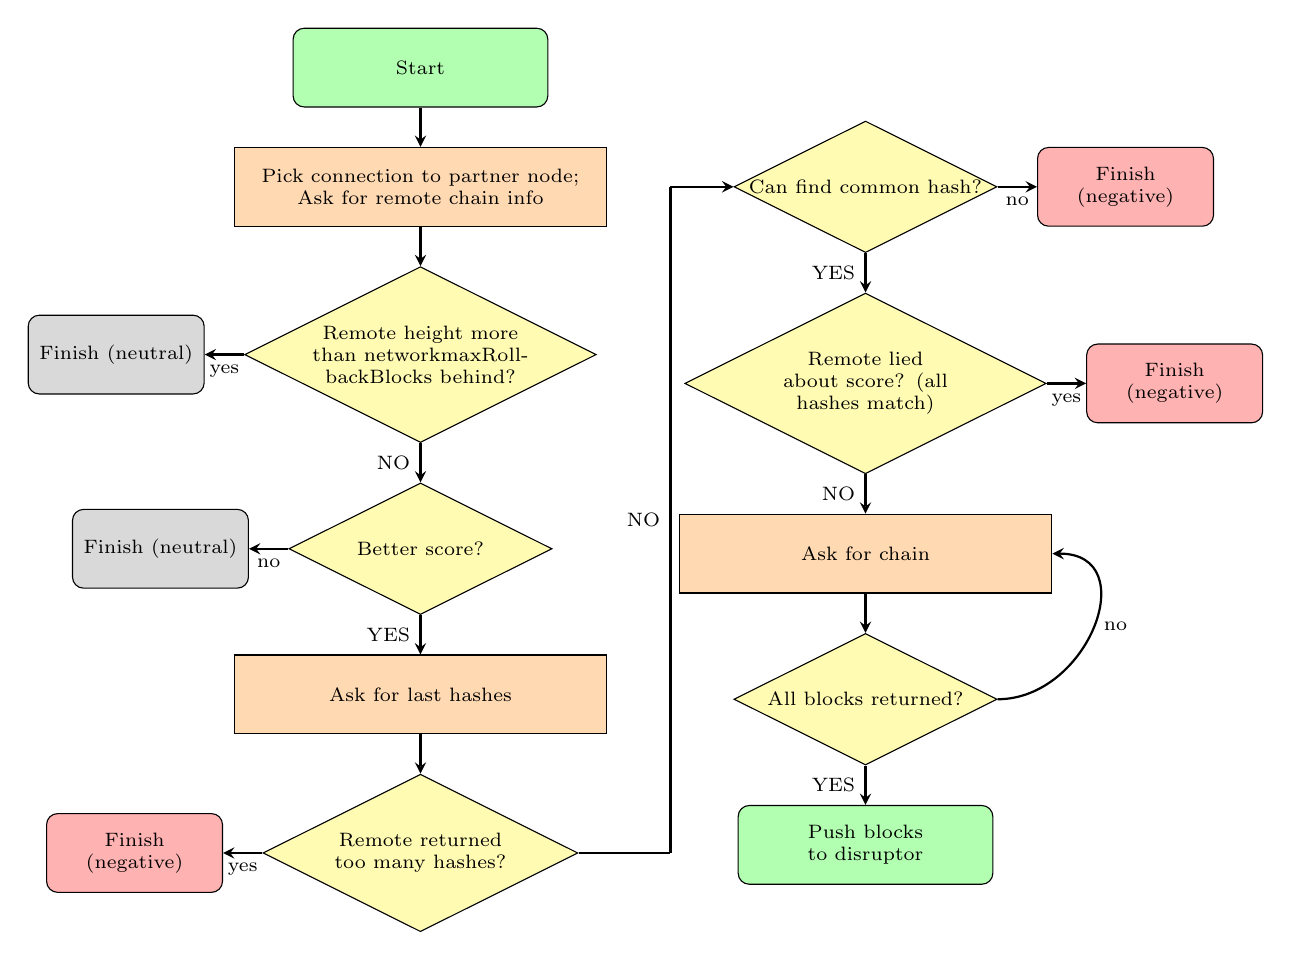
\begin{tikzpicture}[
	node distance=0.5cm and 0.5cm,
	font=\scriptsize
	]
\tikzset{
	base/.style = { rectangle, text centered, draw=black, minimum height=1cm },
	rounded/.style = { base, rounded corners },
	startfinish/.style = { rounded, fill=green!30, minimum width=2cm, text width=3cm },
	finishNeutral/.style = { rounded, fill=gray!30, minimum width=1.5cm, text width=2cm },
	finishNegative/.style = { rounded, fill=red!30, minimum width=1.5cm, text width=2cm },
	finishFailure/.style = { rounded, draw=black, fill=red!30, minimum width=1.5cm, text width=2cm },
	process/.style = { base, text width=4.5cm, fill=orange!30, minimum width=4cm },
	decision/.style = { diamond, text centered, draw=black, minimum height=1cm, aspect=2, text width=3cm, inner sep=0cm, fill=yellow!30, minimum width=2cm },
	arrow/.style ={ thick,->,>=stealth },
	line/.style = { thick,-,>=stealth },
	coord/.style={ coordinate },
	middleSpacing/.style = { xshift=0.3cm }
}

	% left column
	\node (start) [startfinish] {Start};
	\node (remoteScore) [process, below=of start] {Pick connection to partner node; \\ Ask for remote chain info};
	\node (decHeight) [decision, below=of remoteScore] {Remote height more than \nemsetting{network}{maxRollbackBlocks} behind?};
	\node (finishDecHeight) [finishNeutral, left=of decHeight] {Finish (neutral)};

	\node (decRemoteScore) [decision, below=of decHeight] {Better score?};
	\node (finishDecRemoteScore) [finishNeutral, left=of decRemoteScore] {Finish (neutral)};

	\node (remoteHashes) [process, below=of decRemoteScore] {Ask for last hashes};

	\node (decHashesCount) [decision, below=of remoteHashes] {Remote returned too many hashes?};
	\node (finishDecHashesCount) [finishNegative, left=of decHashesCount] {Finish (negative)};

	% invisible helper nodes in the middle
	\node (middleTop) [coord, middleSpacing, right=of remoteScore] {};
	\node (middleBottom) [coord] at (middleTop |- decHashesCount) {};

	% right column
	\node (decHashesCommon) [decision, right=of middleTop, middleSpacing ] {Can find common hash?};
	\node (finishDecHashesCommon) [finishNegative, right=of decHashesCommon] {Finish (negative)};

	\node (decHashesScoreLier) [decision, below=of decHashesCommon] {Remote lied about score? (all hashes match)};
	\node (finishDecHashesScoreLier) [finishNegative, right=of decHashesScoreLier] {Finish (negative)};

	\node (getBlocks) [process, below=of decHashesScoreLier] {Ask for chain};
	\node (decBlocksOk) [decision, below=of getBlocks] {All blocks returned?};

	\node (pushToDisruptor) [startfinish, below=of decBlocksOk] {Push blocks to disruptor};

	% paths
	\draw [arrow] (start) -- (remoteScore);
	\draw [arrow] (remoteScore) -- (decHeight);
	\draw [arrow] (decHeight) -- node[anchor=north] {\scriptsize{yes}} (finishDecHeight);
	\draw [arrow] (decHeight) -- node[anchor=east] {\scriptsize{NO}} (decRemoteScore);

	\draw [arrow] (decRemoteScore) -- node[anchor=north] {\scriptsize{no}} (finishDecRemoteScore);
	\draw [arrow] (decRemoteScore) -- node[anchor=east] {\scriptsize{YES}} (remoteHashes);

	\draw [arrow] (remoteHashes) -- (decHashesCount);
	\draw [arrow] (decHashesCount) -- node[anchor=north] {\scriptsize{yes}} (finishDecHashesCount);

	\draw [line] (decHashesCount) -- (middleBottom);
	\draw [line] (middleBottom) -- node[anchor=east] {\scriptsize{NO}} (middleTop);
	\draw [arrow] (middleTop) -- (decHashesCommon);

	\draw [arrow] (decHashesCommon) -- node[anchor=north] {\scriptsize{no}} (finishDecHashesCommon);
	\draw [arrow] (decHashesCommon) -- node[anchor=east] {\scriptsize{YES}} (decHashesScoreLier);

	\draw [arrow] (decHashesScoreLier) -- node[anchor=north] {\scriptsize{yes}} (finishDecHashesScoreLier);
	\draw [arrow] (decHashesScoreLier) -- node[anchor=east] {\scriptsize{NO}} (getBlocks);

	\draw [arrow] (getBlocks) -- (decBlocksOk);
	\draw (decBlocksOk.0)  edge[arrow, out=0, in=0, looseness=1.5]  node[anchor=west] {\scriptsize{no}} (getBlocks.0);
	\draw [arrow] (decBlocksOk) -- node[anchor=east] {\scriptsize{YES}} (pushToDisruptor);
\end{tikzpicture}

		\caption{Blockchain synchronization flow chart\label{fig:blockchain:synchronizationFlowChart}}
	\end{center}
\end{figure}

	\section{Disruptor}
\label{sec:disruptor}

\nemquote{
Death is the great disruptor. It thrusts us opposite life's mirror, invites our truthful exploration, and reveals the naked truth from which rebirth is possible and we are free to reinvent ourselves anew.
}{B.G. Bowers}

\nemchapterfirstletter{O}{ne} main goal of \codenamespace is to achieve high throughput.
In order to help achieve this goal, the disruptor\footnote{ \url{https://en.wikipedia.org/wiki/Disruptor_(software)} } pattern is used to perform most data processing.
A disruptor uses a ring buffer data structure to hold all elements in need of processing.
New elements are inserted into the next free slot of the ring buffer.
Fully processed elements are removed to make space for new elements.
Since the ring buffer has a finite number of slots, it can run out of space if processing can't keep up with new insertions.
The behavior of \codename, in such a case, can be configured to either to exit the server or discard new data until a slot becomes available.

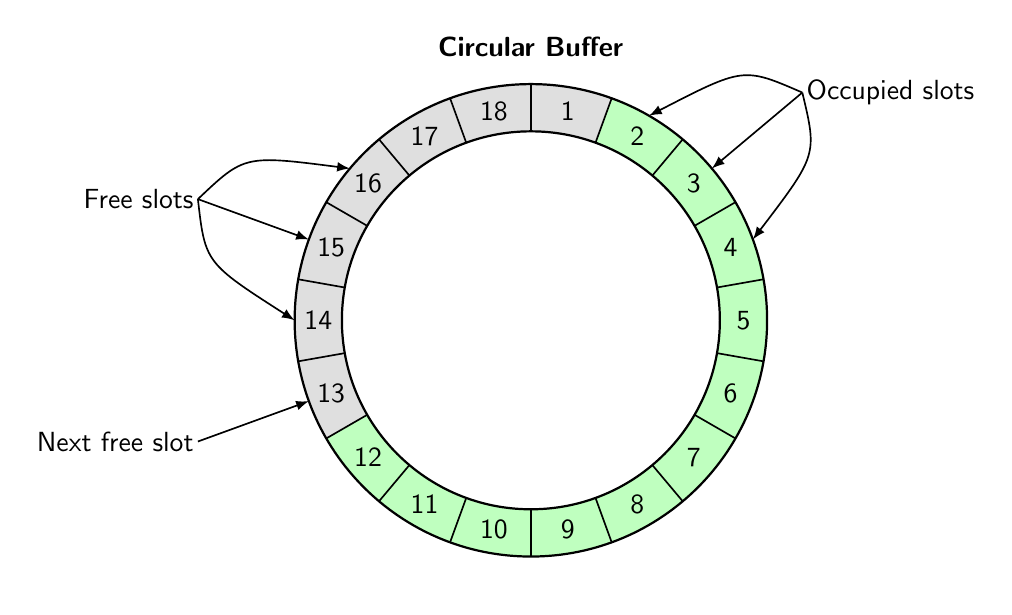
\begin{tikzpicture}[>=latex,font=\sffamily,semithick,scale=3,label distance=-2mm]
	\fill [green!25] (0,0) -- (70:1) arc [end angle=-150, start angle=70, radius=1] -- cycle;
	\fill [gray!25] (0,0) -- (70:1) arc [end angle=210, start angle=70, radius=1] -- cycle;
	\draw [thick,minimum size=6cm] (0,0) circle(1);
	\draw (90:1.1) node[label=above:\textbf{Circular Buffer}]{};
	\foreach \angle in {90,70,...,-70}
		\draw (\angle:1) -- (\angle-180:1);

	\foreach \angle [count=\anglei] in {80,60,...,-260}
		\draw (\angle:0.9) node[] {\anglei};

	\draw [thick,fill=white,minimum size=3cm] (0,0) circle(0.8);

	\draw [->] (160:1.5) .. controls (170:1.4) .. (180:1);
	\draw [->] (160:1.5) -- (160:1);
	\draw [->] (160:1.5) .. controls (150:1.4) .. (140:1);
	\draw [] (160:1.5) node[label=left:Free slots]{};

	\draw [->] (40:1.5) .. controls (50:1.4) .. (60:1);
	\draw [->] (40:1.5) -- (40:1);
	\draw [->] (40:1.5) .. controls (30:1.4) .. (20:1);
	\draw [] (40:1.5) node[label=right:Occupied slots]{};

	\draw [->] (200:1.5) -- (200:1);
	\draw (200:1.5) node[label=left:Next free slot]{};

	(Head.west);
\end{tikzpicture}

Each element in the ring buffer is processed by one or more consumers.
Each consumer takes a single element as input.
Some consumers calculate data from the input and attach it to the element, while others validate the element or alter the global chain state using the element's data.
Some consumers depend on the work done by previous consumers.
Therefore, consumers always need to act on input elements in a predefined order.
To ensure this, each consumer has an associated barrier.
The barrier prevents a consumer from processing an element that has not yet been processed by its immediately preceding consumer.
The last consumer reclaims all memory that was used during processing.
Consumers can set an element's completion status to \textit{Aborted} in case it is already known or invalid for some reason.
Subsequent consumers ignore aborted elements.

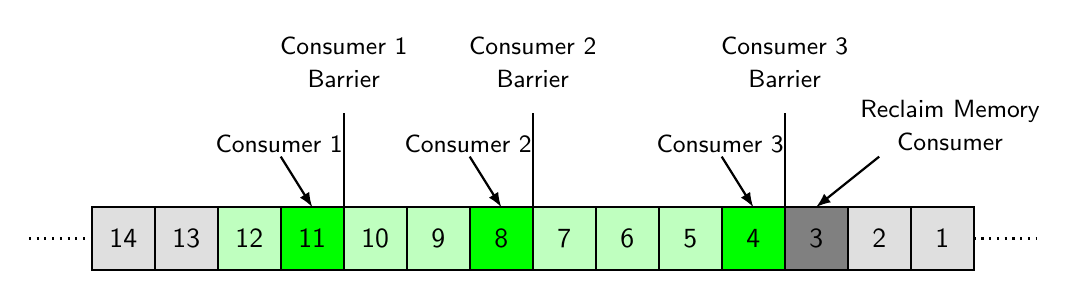
\begin{tikzpicture}[>=latex,font=\sffamily,thick,,scale=0.8]
	% Dots
	\draw[thick,dotted,step=.5] (0,0.5) grid (1,0.5);
	\draw[thick,dotted,step=.5] (15,0.5) grid (16,0.5);

	% Rectangles
	\foreach \i [] in {1,2,13,14}
		\filldraw[draw=black,fill=gray!25] (\i,0) rectangle (\i+1,1);
	\foreach \i [] in {3,5,6,8,9,10}
		\filldraw[draw=black,fill=green!25] (\i,0) rectangle (\i+1,1);
	\foreach \i [] in {4,7,11}
		\filldraw[draw=black,fill=green] (\i,0) rectangle (\i+1,1);
	\filldraw[draw=black,fill=gray] (12,0) rectangle (13,1);

	% Consumer 1
	\draw [] (5,2.0) node[xshift=0.25cm,label=left:\small{Consumer 1}]{};
	\draw [->] (4,1.8) -- (4.5,1);
	\draw [] (5,3.3) node[align=center]{\small{Consumer 1}\\\small{Barrier}};
	\draw [] (5,1) -- (5, 2.5);

	% Consumer 2
	\draw [] (8,2.0) node[xshift=0.25cm,label=left:\small{Consumer 2}]{};
	\draw [->] (7,1.8) -- (7.5,1);
	\draw [] (8,3.3) node[align=center]{\small{Consumer 2}\\\small{Barrier}};
	\draw [] (8,1) -- (8, 2.5);

	% Consumer 3
	\draw [] (12,2.0) node[xshift=0.25cm,label=left:\small{Consumer 3}]{};
	\draw [->] (11,1.8) -- (11.5,1);
	\draw [] (12,3.3) node[align=center]{\small{Consumer 3}\\\small{Barrier}};
	\draw [] (12,1) -- (12, 2.5);

	% Reclaim memory consumer
	\draw [] (13,2.3) node[align=center,xshift=1.3cm]{\small{Reclaim Memory}\\\small{Consumer}};
	\draw [->] (13.5,1.8) -- (12.5,1);

	% Numbers
	\foreach \index [count=\indexi] in {14,13,...,1}
		\draw (\indexi+0.5,0.5) node[] {\index};
\end{tikzpicture}

\subsection{Consumers}
\index{consumers}
\label{sec:disruptor:consumers}
In \codename, a block disruptor is used to process incoming blocks and blockchain parts.
A blockchain part is an input element composed of multiple blocks.
This disruptor is primarily responsible for validating, reconciling and growing the blockchain.

A transaction disruptor is used to process incoming, unconfirmed transactions.
Transactions that are fully processed get added to the unconfirmed transactions cache.

All disruptors are associated with a chain of consumers that perform all processing of their input elements.
Different disruptors are customized by using different consumer chains.
All consumers can inspect the data being processed and some can modify it.

\begin{figure}[H]
	\nemcenterwithcaption{
		\begin{subfigure}{.5\textwidth}
			\nemcenterwithcaption{
				\tikzstyle{consumer} = [rectangle, rounded corners, text centered, draw=black, minimum width=7cm, minimum height=0.5cm, text width=6.5cm]
				\vspace{0pt}
				\begin{tikzpicture}[>=latex,font=\small ,semithick,scale=1,node distance=1.1cm]
					% block consumers
					\node (audit consumer) [consumer] {Audit Consumer (optional)};
					\node (hash calculator consumer) [consumer, below of=audit consumer] {Hash Calculator Consumer};
					\node (hash check consumer) [consumer, below of=hash calculator consumer] {Hash Check Consumer};
					\node (blockchain check consumer) [consumer, below of=hash check consumer] {Blockchain Check Consumer};
					\node (stateless validation consumer) [consumer, below of=blockchain check consumer] {Stateless Validation Consumer};
					\node (batch signature consumer) [consumer, below of=stateless validation consumer] {Batch Signature Consumer};
					\node (blockchain sync consumer) [consumer, below of=batch signature consumer] {Blockchain Sync Consumer};
					\node (blockchain sync cleanup consumer) [consumer, below of=blockchain sync consumer] {Blockchain Sync Cleanup Consumer (optional)};
					\node (new block consumer) [consumer, below of=blockchain sync cleanup consumer] {New Block Consumer};

					% arrows
					\draw [semithick,->] (audit consumer) -- (hash calculator consumer);
					\draw [semithick,->] (hash calculator consumer) -- (hash check consumer);
					\draw [semithick,->] (hash check consumer) -- (blockchain check consumer);
					\draw [semithick,->] (blockchain check consumer) -- (stateless validation consumer);
					\draw [semithick,->] (stateless validation consumer) -- (batch signature consumer);
					\draw [semithick,->] (batch signature consumer) -- (blockchain sync consumer);
					\draw [semithick,->] (blockchain sync consumer) -- (blockchain sync cleanup consumer);
					\draw [semithick,->] (blockchain sync cleanup consumer) -- (new block consumer);
				\end{tikzpicture}
			}{Block Consumers}
		\end{subfigure}%
		\begin{subfigure}{.5\textwidth}
			\nemcenterwithcaption{
				\tikzstyle{consumer} = [rectangle, rounded corners, text centered, draw=black, minimum width=6cm, minimum height=0.6cm, text width=6.5cm]
				\vspace{0pt}
				\begin{tikzpicture}[>=latex,font=\small,semithick,scale=1,node distance=1.1cm]
					% transactions consumers
					\node (audit consumer) [consumer] {Audit Consumer (optional)};
					\node (hash calculator consumer) [consumer, below of=audit consumer] {Hash Calculator Consumer};
					\node (hash check consumer) [consumer, below of=hash calculator consumer] {Hash Check Consumer};
					\node (dummy1) [consumer, below of=hash check consumer, draw=none] {};
					\node (stateless validation consumer) [consumer, below of=dummy1] {Stateless Validation Consumer};
					\node (batch signature consumer) [consumer, below of=stateless validation consumer] {Batch Signature Consumer};
					\node (dummy2) [consumer, below of=batch signature consumer, draw=none] {};
					\node (dummy3) [consumer, below of=dummy2, draw=none] {};
					\node (new transactions consumer) [consumer, below of=dummy3] {New Transactions Consumer};

					% arrows
					\draw [semithick,->] (audit consumer) -- (hash calculator consumer);
					\draw [semithick,->] (hash calculator consumer) -- (hash check consumer);
					\draw [semithick,->] (hash check consumer) -- (stateless validation consumer);
					\draw [semithick,->] (stateless validation consumer) -- (batch signature consumer);
					\draw [semithick,->] (batch signature consumer) -- (new transactions consumer);
				\end{tikzpicture}
			}{Transactions Consumers}
		\end{subfigure}
	}{\codenamespace consumer chains}
\end{figure}

\subsubsection{Common Consumers}
\label{sec:disruptor:commonConsumers}
\index{consumers!common}
The block and transaction disruptors share a number of consumers.

\subsubsection*{Audit Consumer}
This consumer is optional and can be enabled via node configuration.
If enabled, all new elements are written to disk.
This makes it possible to replay the incoming network action and is helpful for debugging.

\subsubsection*{Hash Calculator And Hash Check Consumers}
It is very common for a server to receive the same element many times because networks consist of many servers that broadcast elements to several other servers.
For performance reasons, it is desirable to detect at an early stage whether an element has already been processed in order to avoid processing it again.

The hash calculator consumer calculates all the hashes associated with an element.
The hash check consumer uses the hashes to search the recency cache, which contains the hashes of all recently seen elements.
The consumer used by the transaction disruptor will also search the hash cache (containing hashes of confirmed transactions) and the unconfirmed transactions cache.
If the hash is found in any cache, the element is marked as \textit{Aborted} and further processing is bypassed.

\subsubsection*{Stateless Validation Consumer}
This consumer handles state independent validation by validating each entity in an element.
This can be done in parallel using many threads.
Each plugin can add stateless validators.

An example of a stateless validation is the validation that a block does not contain more transactions than allowed by the network.
This check depends on the network configuration but not on the global blockchain state.

\subsubsection*{Batch Signature Consumer}
This consumer validates all signatures of all entities in an element.
This is separate from the \textit{Stateless Validation Consumer} because it uses batch verification.
For improved performance, this consumer processes many signatures at once in a batch instead of individually.
This can be done in parallel using many threads.

\subsubsection*{Reclaim Memory Consumer}
This consumer completes processing of and frees all memory associated with an element.
It triggers downstream propagation of the statuses of all transactions that were updated during processing.
The overall result of the sync operation is used to update the reputation of - and possibly ban - the sync partner \nemrefparens{sec:reputation}).

\subsubsection{Additional Block Consumers}
\label{sec:disruptor:blockConsumers}
\index{consumers!block}
The block disruptor also uses a few block-specific consumers.

\subsubsection*{Blockchain Check Consumer}
This consumer performs state-independent integrity checks of the chain part contained within an element.
It checks that:
\begin{itemize}
	\item The chain part is not composed of too many blocks.
	\item The timestamp of the last block in the chain part is not too far in the future.
	\item All blocks within the chain part are linked.
	\item There are no duplicate transactions within the chain part.
\end{itemize}

\subsubsection*{Blockchain Sync Consumer}
This consumer is the most complex one.
All tasks that require or alter the local server's chain state are performed in this consumer.

First, it checks that the new chain part can be attached to the existing chain.
If the chain part attaches to a block preceding the tail block, all blocks starting with the tail block are undone in reverse order until the common block is reached.

Next, it executes each block by performing stateful validation and then observing changes.
Stateless validation is skipped because it was performed by previous consumers.
If there are any validation failures, the entire chain part is rejected.
Otherwise, all changes are committed to the chain state (both the block and cache storages) and the unconfirmed transactions cache is updated.

\emph{This consumer is the only part of the \codenamespace system that modifies the chain state and needs write access to it.}

\subsubsection*{Blockchain Sync Cleanup Consumer}
This consumer is optional and can be enabled via node configuration.
If enabled, it removes all files that were created by the \textit{Blockchain Sync Consumer}.
This consumer should only be enabled when a server is running without a broker.

\subsubsection*{New Block Consumer}
This consumer forwards single blocks, either harvested by the server or pushed from a remote server, to other servers in the network.

\subsubsection{Additional Transaction Consumers}
\label{sec:disruptor:transactionConsumers}
\index{consumers!transaction}
The transaction disruptor uses a single transaction-specific consumer.

\subsubsection*{New Transactions Consumer}
This consumer forwards all transactions that have valid signatures and have passed stateless validation to the network.
Stateful validation is not performed on transactions until they're added to the unconfirmed transactions cache.
Forwarding is intentionally done before stateful validation because one server might reject transactions that could be accepted by other servers (e.g. if the transaction has too low a fee for the local server).
Subsequently, stateful validation is performed on the forwarded transactions, and the valid ones are stored in the unconfirmed transactions cache.

	\section{Unconfirmed Transactions}
\label{sec:unconfirmedTransactions}

\nemquote{
}{}

\nemchapterfirstletter{A}{ny} transaction that is not yet included in a block is called an \textit{unconfirmed transaction}.
These transactions may be valid or invalid.
Valid unconfirmed transactions are eligible for inclusion in a harvested block.
Once a transaction is added to a block that is accepted in the blockchain, it is \textit{confirmed}.

Unconfirmed transactions can arrive at a node when:
\begin{enumerate}
	\item{A client sends a new transaction directly to the node.}
	\item{A bonded aggregate transaction is completed with all requisite cosignatures and is promoted from the partial transactions cache.}
	\item{A peer node broadcasts transactions to the node.}
	\item{A peer node responds to the node's request for unconfirmed transactions.
	As an optimization, the requesting node indicates what transactions it already knows in order to avoid receiving redundant transactions.
	Additionally, it supplies the minimum fee multiplier \nemrefparens{sec:blockchain:generation} it uses when creating blocks.
	This prevents the remote node from returning unconfirmed transactions that will be immediately rejected by the requesting node.}
\end{enumerate}

When an unconfirmed transaction arrives at a node, it is added to the transaction disruptor \nemrefparens{sec:disruptor}.
All transactions that haven't been previously seen and pass stateless validation will be broadcast to peer nodes.
At this point, it is still possible for the node to reject the broadcast transactions because stateful validation is performed after broadcasting.
Due to different node settings, it's possible for some nodes to accept a specific unconfirmed transaction and other nodes to reject it.
For example, the nodes could have different \nemsetting{node}{minFeeMultiplier} settings.

\subsection{Unconfirmed Transactions Cache}
\index{unconfirmedTransactions!cache}

When a transaction passes all validation, it is eligible for inclusion in a harvested block.
At this point, the node tries to add it to the \textit{unconfirmed transactions cache}.
This can fail for two reasons:
\begin{enumerate}
	\item{The maximum cache size configured by \nemsetting{node}{unconfirmedTransactionsCacheMaxSize} has been reached.}
	\item{The cache contains at least as many unconfirmed transactions as can be included in a single block and the new transaction is rejected by the Spam throttle}.
\end{enumerate}

Whenever new blocks are added to the blockchain, the blockchain state changes and the unconfirmed transactions cache is affected.
Although all transactions in the cache are valid at the time they were added, this doesn't guarantee that they'll be valid in perpetuity.
For example, a transaction could have already been included in a block harvested by another node or a conflicting transaction could have been added to the blockchain.
This means that transactions in the cache that were perfectly valid previously could be invalidated after changes to the blockchain state.
Additionally, when blocks with transactions are reverted, it's possible that some of those previously confirmed transactions are no longer included in any block in the new chain.
Those reverted transaction should be added to the cache.

As a result of these considerations, the entire unconfirmed transactions cache is completely rebuilt whenever the blockchain changes.
Each transaction is rechecked by the stateful validators and purged if it has become invalid or has already been included in a block.
Otherwise, it is added back to the cache.

\subsection{Spam Throttle}
\index{unconfirmedTransactions!spamThrottle}

The initiator of an unconfirmed transaction does not have to pay a fee to nodes holding the transaction in the unconfirmed transactions cache.
Since the cache uses valuable resources, a node must have some protection against being spammed with lots of unconfirmed transactions.
This is especially important if the node is generous and accepts zero fee transactions.

Simply limiting the number of unconfirmed transactions that a node accepts is suboptimal because normal actors should still be able to send a transaction even when a malicious actor is spamming the network.
Limiting the number of unconfirmed transactions per account is also not a good option because accounts are free to create.

\codenamespace implements a smart throttle that prevents an attacker from filling the cache completely with transactions while still letting honest actors successfully submit new unconfirmed transactions.
\nemsetting{node}{enableTransactionSpamThrottling} can be used to activate the throttle.
Assuming the cache is not full, it works in the following way:
\begin{enumerate}
	\item{If the cache contains fewer unconfirmed transactions than can be included in a single block, throttling is bypassed.}
	\item{If the new transaction is a bonded aggregate transaction, throttling is bypassed.}
	\item{Else the Spam throttle is applied.}
\end{enumerate}

Let \textit{curSize} be the current number of transactions in the cache and \textit{maxSize} the configured maximum size of the cache.
Also let \textit{rel. importance of A} be the relative importance of $A$, i.e. a number between 0 and 1.
If a new unconfirmed transaction with signer $A$ arrives, then the \textit{fair share} for account $A$ is calculated:
\begin{align*}
	\textit{maxBoostFee} &= \text{\nemsetting{node}{transactionSpamThrottlingMaxBoostFee}} \\
	\textit{maxFee} &= \min(\textit{maxBoostFee}, \structField{transaction}{MaxFee}) \\
	\textit{eff. importance} &= (\textit{rel. importance of A}) + 0.01 \cdot \frac{\textit{maxFee}}{\textit{maxBoostFee}} \\
	\textit{fair share} &= 100 \cdot (\textit{eff. importance}) \cdot (\textit{maxSize} - \textit{curSize}) \cdot \exp\left(-3 \frac{\textit{curSize}}{\textit{maxSize}}\right)
\end{align*}

If account $A$ already has as many transactions in the cache as its fair share, then the new transaction is rejected.
Otherwise, it is accepted.
The formula shows that an increase in a transaction's maximum fee increases the number of slots available in the cache.
Nonetheless, this mechanism for boosting the effective importance is limited by \nemsetting{node}{transactionSpamThrottlingMaxBoostFee}.

\begin{figure}[ht]
	\nemcenterwithcaption{
		\pgfplotsset{
			legend entry/.initial=,
			every axis plot post/.code={%
				\pgfkeysgetvalue{/pgfplots/legend entry}\tempValue
				\ifx\tempValue\empty
					\pgfkeysalso{/pgfplots/forget plot}%
				\else
					\expandafter\addlegendentry\expandafter{\tempValue}%
				\fi
			},
		}
		\begin{tikzpicture}[trim axis left]
			\begin{axis}[
					scale only axis,
					xlabel = \text{cache fill level [\%]},
					xticklabel={\pgfmathparse{int(\tick / 100)}\pgfmathprintnumber{\pgfmathresult}},
					scaled x ticks=false,
					ylabel = fair share,
					height = 5cm,
					width=(4 * \textwidth) / 5
				]
				\addplot[color=blue,domain=1500:10000,legend entry=$0.01\%$]{100 * 0.0001 * (10000 - x) * exp(-3 * x / 10000)};
				\addplot[color=red,domain=1500:10000,legend entry=$0.005\%$]{100 * 0.00005 * (10000 - x) * exp(-3 * x / 10000)};
				\addplot[color=green,domain=1500:10000,legend entry=$0.001\%$]{100 * 0.00001 * (10000 - x) * exp(-3 * x / 10000)};
			\end{axis}
		\end{tikzpicture}
	}{Fair share for various effective importances with max cache size = 10000}
	\label{fig:unconfirmedTransactions:fairShare}
\end{figure}

\autoref{fig:unconfirmedTransactions:fairShare} shows the fair share of slots relative to the fill level of the cache for various effective importances.
An attacker that tries to occupy many slots cannot gain much by using many accounts because the importance of each account will be very low.
The attacker can increase maximum transaction fees but that will be more costly and expend funds at a faster rate.

	\section{Partial Transactions}
\label{sec:partials}

\nemquote{
Lorem ipsum
}{}

\nemchapterfirstletter{B}{onded} aggregate transactions \nemrefparens{sec:transactions:aggregate} are also referred to as partial transactions.
The name \emph{partial} is fitting because the transactions have insufficient cosignatures and are unable to pass validation until more cosignatures are collected.

Support for handling partial transactions is provided by the \textit{partial transaction extension}.
If a network supports bonded aggregate transactions, this extension should be enabled on all Api and Dual nodes.

Partial transactions are synchronized among all nodes in a network that have this extension enabled.
A node passively receives partial transactions and cosignatures pushed by remote nodes.
It also periodically requests transactions and cosignatures from remote nodes via the \textit{pull partial transactions task}.
As an optimization, the requesting node indicates which transactions and cosignatures it already knows in order to avoid receiving redundant information.

When the hash lock plugin is enabled, in order for a partial transaction to be accepted by the network, a hash lock must be created and associated with the transaction.
The hash lock is essentially a bond paid in order to use the built-in cosignature collection service.
If the associated partial transaction is completed and confirmed in the blockchain before the hash lock expires, the bond is returned to the payer.
Otherwise, the bond is forfeited to the harvester of the block at which the lock expires.
This feature makes spamming the partial transactions cache more costly because it requires \nemsetting{node}{lockedFundsPerAggregate} to be paid, at least temporarily, for a partial transaction to enter the cache.

When a node receives a new partial transaction, it is pushed to the \textit{partial transaction dispatcher}.
Received cosignatures are collated with partial transactions already in the cache and are immediately rejected if there are no matching transactions
\footnote{This implies that a partial transaction must be present in the cache before any of its cosignatures can be accepted.}.
When transactions and cosignatures are received together, they are split and processed individually as above.

Compared to the normal transaction dispatcher \nemrefparens{sec:disruptor:consumers}, the partial transaction dispatcher is minimalistic.

\begin{figure}[H]
	\nemcenterwithcaption{
		\tikzstyle{consumer} = [rectangle, rounded corners, text centered, draw=black, minimum width=7cm, minimum height=0.5cm, text width=6.5cm]
		\vspace{0pt}
		\begin{tikzpicture}[>=latex,font=\small ,semithick,scale=1,node distance=1.1cm]
			% consumers
			\node (hash calculator consumer) [consumer, below of=audit consumer] {Hash Calculator Consumer};
			\node (hash check consumer) [consumer, below of=hash calculator consumer] {Hash Check Consumer};
			\node (new transactions consumer) [consumer, below of=hash check consumer] {New Transactions Consumer};

			% arrows
			\draw [semithick,->] (hash calculator consumer) -- (hash check consumer);
			\draw [semithick,->] (hash check consumer) -- (new transactions consumer);
		\end{tikzpicture}
	}{Partial transaction consumers}
\end{figure}

The hash calculator and hash check consumers work as described for the transaction dispatcher in \nemref{sec:disruptor:commonConsumers}.
The one difference is that the hash check consumer will additionally search the partial transactions cache for previously seen transactions.
The new transaction consumer has a similar purpose to the one described in \nemref{sec:disruptor:transactionConsumers}.
The difference is that it broadcasts and processes partial transactions instead of unconfirmed transactions.
Specifically, it broadcasts partial transactions to the network and then adds valid ones to the partial transactions cache.

\subsection{Partial Transaction Processing}
\label{sec:partials:processing}

The partial transactions cache contains all partial transactions that are waiting for additional cosignatures.
When a new partial transaction is received that passes all validation, it is added to the cache.
It will stay in the cache until a sufficient number of cosignatures are collected or it becomes invalid.
For example, the transaction will be purged if its associated hash lock expires.
Whenever a partial transaction is completed by collecting sufficient cosignatures, it will immediately be forwarded to the transaction dispatcher and be processed as an unconfirmed transaction.

\begin{figure}
	\nemcenterwithcaption{
		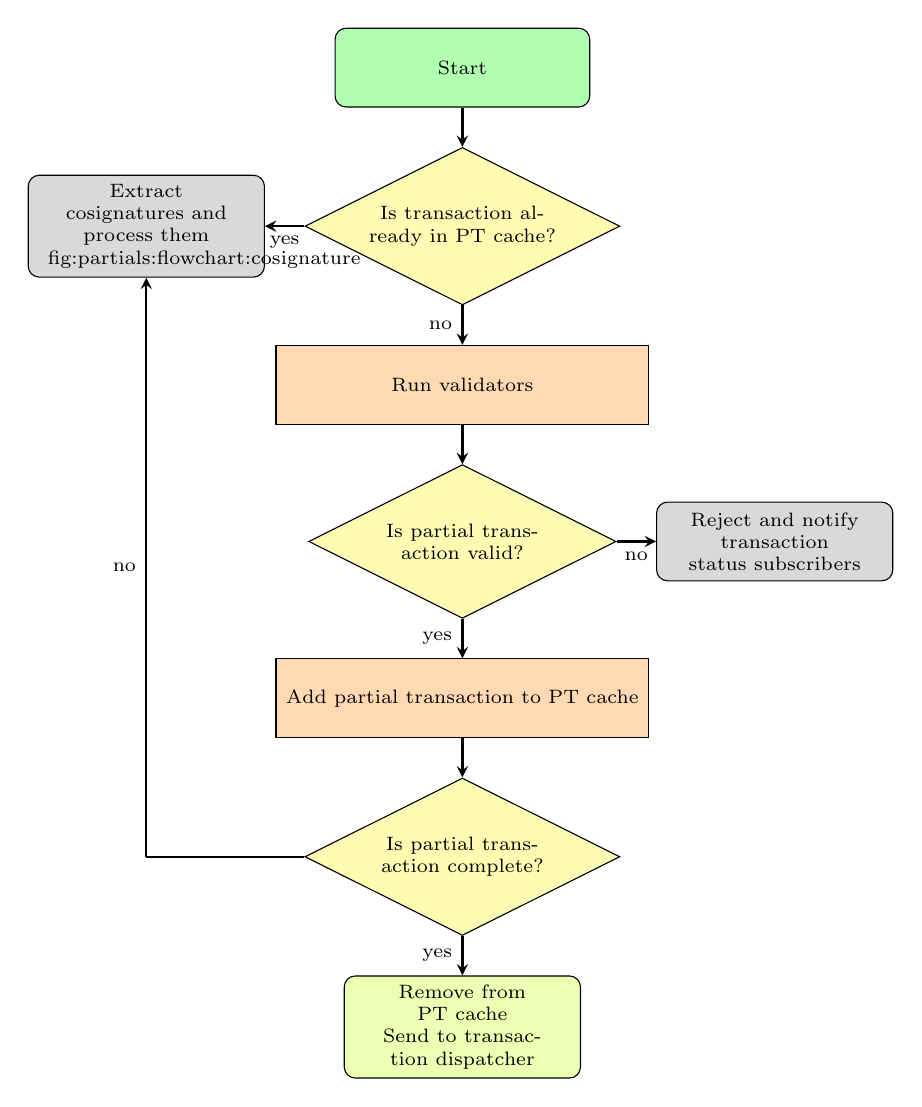
\begin{tikzpicture}[
	node distance=0.5cm and 0.5cm,
	font=\scriptsize
	]
\tikzset{
	base/.style = { rectangle, text centered, draw=black, minimum height=1cm },
	rounded/.style = { base, rounded corners },
	startfinish/.style = { rounded, fill=green!30, minimum width=2cm, text width=3cm },
	finish/.style = { rounded, fill=gray!30, minimum width=3cm, text width=2.5cm },
	process/.style = { base, text width=4.5cm, fill=orange!30, minimum width=4cm },
	decision/.style = { diamond, text centered, draw=black, minimum height=1cm, aspect=2, text width=3cm, inner sep=0cm, fill=yellow!30, minimum width=2cm },
	arrow/.style ={ thick,->,>=stealth },
	line/.style = { thick,-,>=stealth },
	coord/.style={ coordinate },
	middleSpacing/.style = { xshift=0.3cm }
}

	% left column
	\node (start) [startfinish] {Start};
	\node (decCache) [decision, below=of start] {Is transaction already in PT cache?};
	\node (finishDecCache) [finish, left=of decCache] {Extract cosignatures and process them \nemrefparens{fig:partials:flowchart:cosignature}};

	\node (runValidators) [process, below=of decCache] {Run validators};
	\node (decValid) [decision, below=of runValidators] {Is partial transaction valid?};
	\node (finishInvalid) [finish, right=of decValid] {Reject and notify transaction status subscribers};

	\node (addToCache) [process, below=of decValid] {Add partial transaction to PT cache};
	\node (decComplete) [decision, below=of addToCache] {Is partial transaction complete?};
	\node (leftBottom) [coord] at (finishDecCache |- decComplete) {};

	\node (finishComplete) [finish, fill=lime!30, below=of decComplete] {Remove from PT cache \\ Send to transaction dispatcher};

	% paths
	\draw [arrow] (start) --  (decCache);
	\draw [arrow] (decCache) -- node[anchor=north] {\scriptsize{yes}} (finishDecCache);
	\draw [arrow] (decCache) -- node[anchor=east] {\scriptsize{no}} (runValidators);

	\draw [arrow] (runValidators) -- (decValid);
	\draw [arrow] (decValid) -- node[anchor=north] {\scriptsize{no}} (finishInvalid);
	\draw [arrow] (decValid) -- node[anchor=east] {\scriptsize{yes}} (addToCache);

	\draw [arrow] (addToCache) -- (decComplete);

	\draw [line] (decComplete) -- (leftBottom);
	\draw [arrow] (leftBottom) -- node[anchor=east] {\scriptsize{no}} (finishDecCache);

	\draw [arrow] (decComplete) -- node[anchor=east] {\scriptsize{yes}} (finishComplete);
\end{tikzpicture}

	}{Processing of a partial transaction}
\end{figure}

The partial transactions cache collates all new cosignatures with the transactions it already contains.
In order to be added to the cache, a cosignature must be new, verifiable and associated with an existing partial transaction.
It is possible for a previously accepted cosignature to become invalid, in which case it should be purged.
For example, a cosignature could become invalid if its signer was removed from a multisignature account participating in the partial transaction.
The cosignature collation process is intricate enough to handle such edge cases.

\begin{figure}
	\nemcenterwithcaption{
		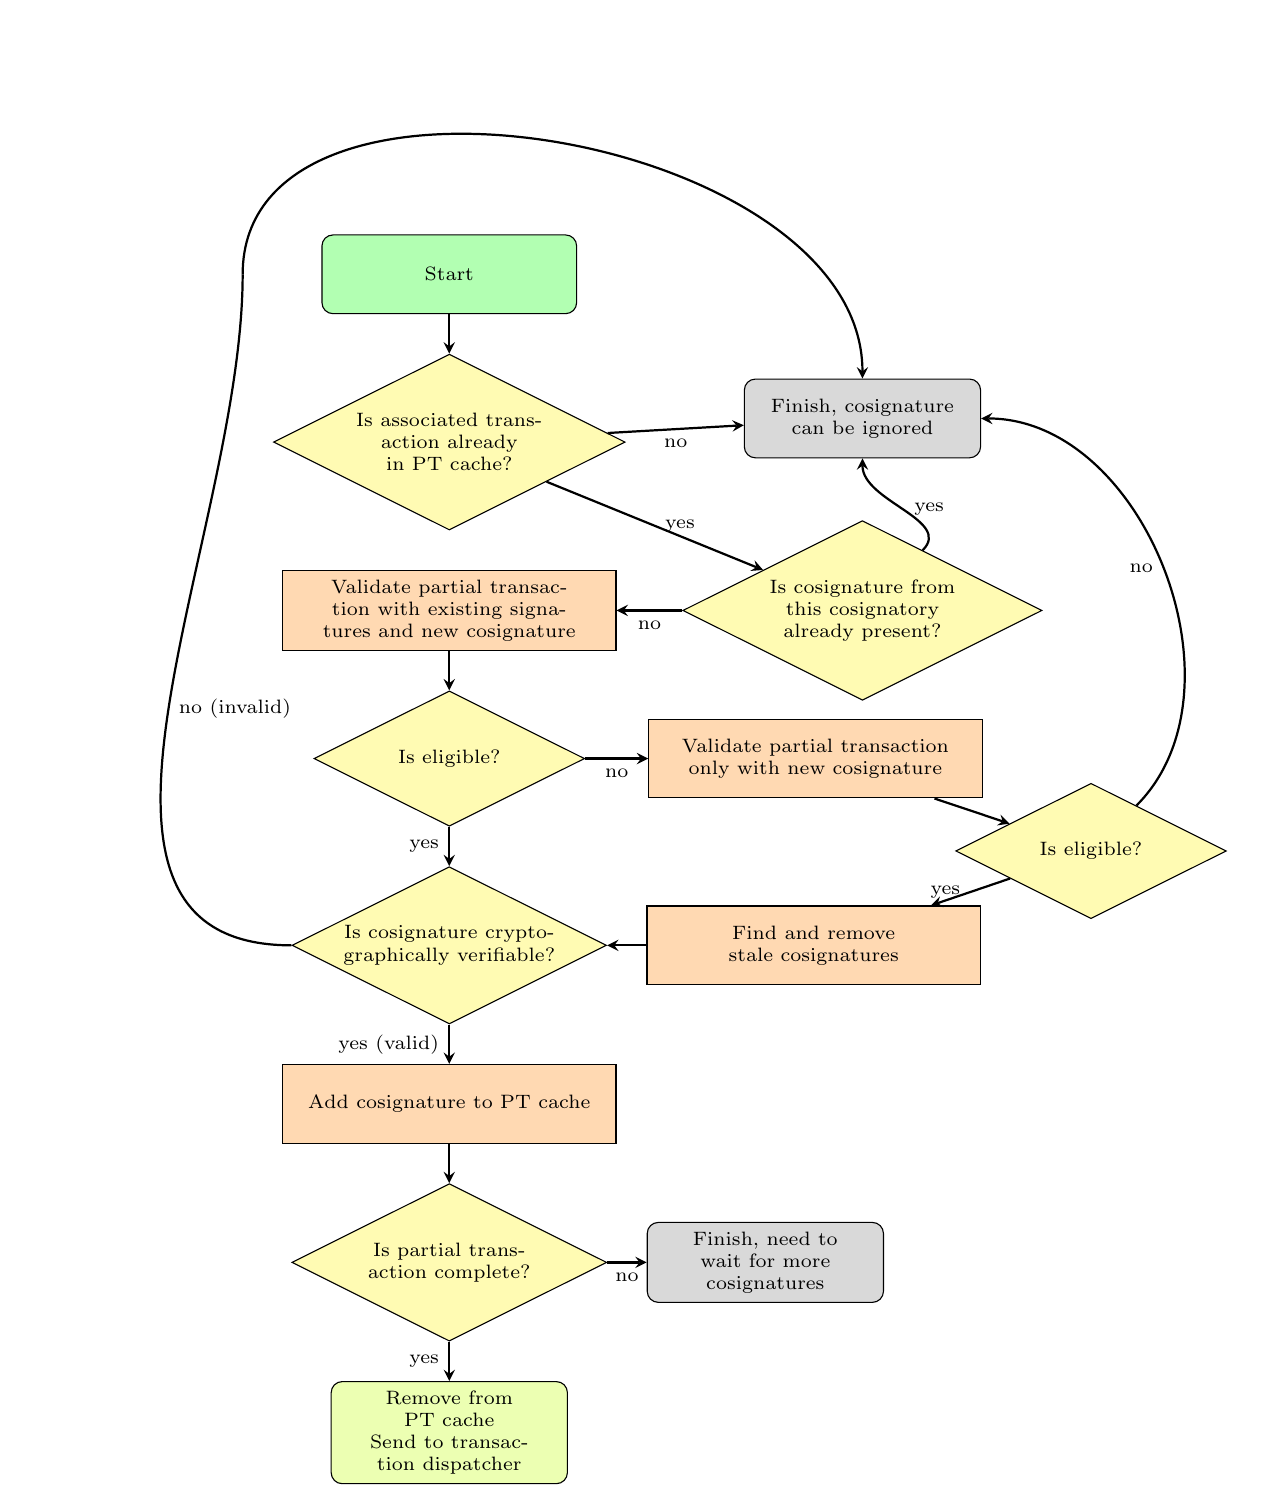
\begin{tikzpicture}[
	node distance=0.5cm and 0.5cm,
	font=\scriptsize
	]
\tikzset{
	base/.style = { rectangle, text centered, draw=black, minimum height=1cm },
	rounded/.style = { base, rounded corners },
	startfinish/.style = { rounded, fill=green!30, minimum width=2cm, text width=3cm },
	finish/.style = { rounded, fill=gray!30, minimum width=3cm, text width=2.5cm },
	process/.style = { base, text width=4cm, fill=orange!30, minimum width=4cm },
	decision/.style = { diamond, text centered, draw=black,aspect=2, text width=3cm, inner sep=0cm, fill=yellow!30 },
	arrow/.style ={ thick,->,>=stealth },
	line/.style = { thick,-,>=stealth },
	coord/.style={ coordinate },
	middleSpacing/.style = { xshift=0.3cm }
}
	% main column
	\node (start) [startfinish] {Start};
	\node (decCache) [decision, below=of start] {Is associated transaction already in PT cache?};
	\node (finishIgnore) [finish, right=of decCache, xshift=1cm, yshift=0.3cm] {Finish, cosignature can be ignored};

	\node (validateCosigI) [process, below=of decCache] {Validate partial transaction with existing signatures and new cosignature};

	\node (decRedundant) [decision] at (validateCosigI -| finishIgnore) {Is cosignature from this cosignatory already present?};

	\node (decEligibleI) [decision, below=of validateCosigI] {Is eligible?};

	\node (decVerifyCosig) [decision, below=of decEligibleI] {Is cosignature cryptographically verifiable?};

	\node (addToCache) [process, below=of decVerifyCosig] {Add cosignature to PT cache};
	\node (decComplete) [decision, below=of addToCache] {Is partial transaction complete?};
	\node (finishWait) [finish, right=of decComplete] {Finish, need to wait for more cosignatures};

	\node (finishComplete) [finish, fill=lime!30, below=of decComplete] {Remove from PT cache \\ Send to transaction dispatcher};

	% side column
	\node (validateCosigE) [process, middleSpacing, right=of decEligibleI] {Validate partial transaction only with new cosignature};
	\node (decEligibleE) [decision, below=of validateCosigE, yshift=0.7cm,  xshift=3.5cm] {Is eligible?};

	\node (removeStale) [process, right=of decVerifyCosig] {Find and remove stale cosignatures};

	% paths
	\draw [arrow] (start) --  (decCache);
	\draw [arrow] (decCache) -- node[anchor=north] {\scriptsize{no}} (finishIgnore);
	\draw [arrow] (decCache) -- node[anchor=west] {\scriptsize{yes}} (decRedundant);

	\draw [arrow] (decRedundant) edge[arrow, in=-90] node[anchor=west] {\scriptsize{yes}} (finishIgnore);
	\draw [arrow] (decRedundant) -- node[anchor=north] {\scriptsize{no}} (validateCosigI);

	\draw [arrow] (validateCosigI) -- (decEligibleI);
	\draw [arrow] (decEligibleI) -- node[anchor=north] {\scriptsize{no}} (validateCosigE);
	\draw [arrow] (decEligibleI) -- node[anchor=east] {\scriptsize{yes}} (decVerifyCosig);

	\node (topLeft) [coord, left=of start, xshift=-0.5cm] {};

	\draw [line] (decVerifyCosig) edge[out=180, in=-90] node[anchor=west] {\scriptsize{no (invalid)}} (topLeft);
	\draw [line] (topLeft) edge[arrow, out=90, in=90] (finishIgnore);

	\draw [arrow] (decVerifyCosig) -- node[anchor=east] {\scriptsize{yes (valid)}} (addToCache);

	\draw [arrow] (addToCache) -- (decComplete);

	\draw [arrow] (decComplete) -- node[anchor=north] {\scriptsize{no}} (finishWait);
	\draw [arrow] (decComplete) -- node[anchor=east] {\scriptsize{yes}} (finishComplete);

	% side column paths
	\draw [arrow] (validateCosigE) -- (decEligibleE);
	\draw [arrow] (decEligibleE) edge[arrow, in=0] node[anchor=east] {\scriptsize{no}} (finishIgnore);
	\draw [arrow] (decEligibleE) -- node[anchor=east] {\scriptsize{yes}} (removeStale);

	\draw [arrow] (removeStale) -- (decVerifyCosig);

\end{tikzpicture}

	}{Processing of a cosignature}
	\label{fig:partials:flowchart:cosignature}
\end{figure}

	\section{Network}
\label{sec:network}

\nemquote{
}{}

\nemchapterfirstletter{D}{ynamic} discovery of nodes allows a peer-to-peer network to grow.
\codenamespace implements this dynamic discovery in the \emph{node discovery extension}.
Public networks are typically open and allow any node to join.
Private networks can restrict the nodes that are allowed to join and behave as a federated system
\footnote{
	By carefully distributing harvesting and currency mosaics, a private network can delegate permissions to different accounts.
	For example, only accounts owning sufficient harvesting mosaic can create blocks and only accounts with nonzero currency can initiate transactions with nonzero fees.
}.
\codenamespace is flexible enough to even allow private networks to specify all node relationships via configuration files.

\subsection{Beacon Nodes}

A freshly booted node is initially isolated and not connected with any peers.
It needs to join a network before it can make any meaningful contributions, like validating or harvesting blocks.
In \codename, nominally \textit{static} beacon nodes are stored in a peers configuration file.
In order to join a network, a new node first connects to these nodes.
These files don't need to be identical across all nodes in a network.

A public network is recommended to specify a set of high availability beacon node candidates.
Each node's peers configuration file should contain a random subset of these nodes.
This reduces stress on individual beacon nodes and makes DoS attacks on beacon nodes more difficult.
These nodes are given slight preference in node selection \nemrefparens{sec:reputation:NodeSelection} relative to non-beacon nodes because they are assumed to have high-availability.
They aren't conferred any other special privileges or responsibilities.
They can be thought of as doors into the network.

Certain extensions may require their own set of beacon nodes.
For example, the \emph{partial transaction extension} stores its own set of beacon nodes in a separate peers configuration file.
Nodes with this extension enabled need to additionally synchronize partial transactions among other nodes that also have this extension enabled  \nemrefparens{sec:partials}.

A node's roles specify the capabilities it supports.
Typically, these are used by a connecting node to choose appropriate partners.
Nodes with the \texttt{Peer} role support basic synchronization.
Nodes with the \texttt{Api} role support partial transaction synchronization.
Roles are not mutually exclusive.
Nodes are allowed to support multiple roles.

\subsection{Connection Handshake}

When two \codenamespace nodes connect with each other, they first perform a two-party custom handshake.
If either node fails the handshake, the connection is immediately terminated.
The primary purpose of this handshake is for each node to prove ownership of its \nemsetting{user}{bootPrivateKey}.
Partner nodes use this verified identity to collate reputation \nemrefparens{sec:reputation} information
\footnote{In the public network, nodes are primarily identified by their resolved IP.}.

Potential vulnerabilities in the \codenamespace proprietary handshake protocol have been identified by penetration testing.
In light of these, the protocol needs to undergo a more thorough review and potential changes.
This section will be updated once a corrective plan is prepared.

\subsection{Packets}

\codenamespace uses TCP for network communication on the port specified by \nemsetting{node}{port}.
Communication is centered around a higher level \emph{packet} model on top of and distinct from TCP packets.
All packets begin with an 8-byte header that specifies each packet's size and type.
Once a complete packet is received, it is ready for further processing.

\begin{figure}[H]
	\nemcenter{
		\nemmemorylayout{
				\begin{leftwordgroup}{\texttt{0x00}}
					\bitbox{4}{Size} \bitbox{4}{Type}
				\end{leftwordgroup} \\
		}{Packet header binary layout}
	}{}
\end{figure}

A mix of long lived and short lived connections are used.
Long lived connections are used for repetitive activities like syncing blocks or transactions.
They support both push and request/response semantics.
The connections are allowed to last for \nemsetting{node}{maxConnectionAge} selection rounds \nemrefparens{sec:reputation:ConnectionManagement} before they are eligible for recycling.
Connections older than this setting are recycled primarily to allow direct interactions with other partner nodes and secondarily as a precaution against zombie connections.

Short lived connections are used for more complex multistage interactions between nodes.
For example, they are used for node discovery \nemrefparens{sec:network:discovery} and time synchronization \nemrefparens{sec:timesync}.
Short lived connections help prevent sync starvation, which can occur when all long lived connections are in use and no sync partners are available.

\emph{Handlers} are used to process packets.
Each handler is registered to accept all packets with a specified packet type.
When a complete packet is ready for processing, it is dispatched to the handler registered with its type.
All handlers must accept matching packets for processing.
Some handlers can also write response packets in order to allow request/response protocols.

\subsection{Connection Types}

In \codename, long lived connections are primarily identified as readers or writers.
This is orthogonal to whether they are incoming or outgoing.
They are secondarily identified by purpose, or \emph{service identifier}
\footnote{Although the terminology is similar, these are unrelated to services described in \nemref{sec:system:extensions}.}.
This allows connections to be selected by capability and more granular logging.

Reader connections are mostly passive and used to receive data from other nodes.
Each server asynchronously reads from each reader connection.
Whenever a new packet is received in its entirety, it is dispatched to an appropriate handler.
If no matching handler is available, the connection is closed immediately.

The \nemsetting{node}{maxIncomingConnectionsPerIdentity} limit is applied across all services and long and short lived connections.
Any incoming connections above this limit will be immediately closed.
This limit can be hit when multiple short lived connections are initiated with the same remote for different operations.
This is more likely when connection tasks are more aggressively scheduled immediately after a node boots up.
These errors are typically transient and can be safely ignored if they don't persist.

Writer connections are more active and used to send data to other nodes.
\emph{Broadcast} operations push data to all active and available writers.
Additionally, individual writers can be checked out and be used for request/response protocols.
In order to simplify recipient processing, no broadcast packets are sent to checked out writers.

Service identifiers are only assigned to long lived connections.
Sync service is used to manage outgoing connections to nodes with \texttt{Peer} role.
Api partial service is used to manage outgoing connections to nodes with \texttt{Api} role.
Readers service is used to manage incoming connections.
Api writers service is experimental and allows incoming connections on port \nemsetting{node}{apiPort} to register as writers.

\begin{figure}[H]
	\nemcenterwithcaption{
		\begin{tabular}{|c|c|c|}
			\hline
			Identifier & Name & Direction\\
			\hline
			0x41504957 & api.writers & incoming \\
			0x50415254 & api.partial & outgoing \\
			0x52454144 & readers & incoming \\
			0x53594E43 & sync & outgoing \\
			\hline
		\end{tabular}
	}{Service Identifiers}
	\label{tbl:network:serviceIdentifiers}
\end{figure}

For the purposes of node selection described in \nemref{sec:reputation:NodeSelection}, node aging and selection are both scoped per service.
Reputational information is aggregated across all services.
Specifically, assume a node has made both a Sync and Api partial connection to another node.
Each connection can have a different age because age is scoped per service.
Interaction results, from any connection, are always attributed to the node, not the service.

\subsection{Peer Provenance}

A node collects data about all nodes in its network.
The reputability of the data is dependent on its provenance.
Possible provenances, ranked from best to worst are:
\begin{enumerate}
	\item{Local - Node is specified in \nemsetting{node}{localnode}}
	\item{Static - Node is in one of the peers configuration files}
	\item{Dynamic - Node was discovered and supports connections}
	\item{Dynamic Incoming - Node has made a connection but does not support connections}
\end{enumerate}

It is important to note that the distinguishing characteristic of a \emph{static} node is that it appears in at least one peers configuration file.
Excepting the \emph{local} node, all other nodes are \emph{dynamic}.
A subset of dynamic nodes are \emph{incoming}.
These nodes have only been seen in incoming but not outgoing connections.
As a result, their preferred port is unknown and they can't be connected with.

Existing node data can only be updated if the new data does not have worse provenance than the existing data.
For example, updated information about a static node with dynamic provenance is discarded, but updated information about a dynamic node with dynamic or static provenance is allowed.

When \nemsetting{network}{nodeEqualityStrategy} is \texttt{public-key}, the secondary identity component is the resolved IP.
When there are no active connections, this is allowed to change.
This strategy does not support reputational migration.

When \nemsetting{network}{nodeEqualityStrategy} is \texttt{host}, the secondary identity component is the public boot key.
When there are no active connections, this is allowed to change.
The resolved IP primary identity component can also be changed when there are no active connections assuming the secondary identity component is unchanged.
In this case, all reputation data associated with the original host is migrated to the new host.
When there is an ambiguous match, data with the matching primary identity component is migrated and data with the matching secondary identity component is discarded.

\subsection{Node Discovery}
\label{sec:network:discovery}

\codenamespace supports a configurable node identification policy configured by \nemsetting{network}{nodeEqualityStrategy}.
Valid policies allow identifying a node by either its \textit{resolved IP} (\texttt{host})
\footnote{
	A node's resolved IP is only broadcast to other nodes when it doesn't specify a hostname.
	Hostnames are preferentially propagated in order to support nodes with dynamic IPs.
}or \textit{public boot key} (\texttt{public-key}).
The former is preferred for public networks.

After starting up, a node attempts to make short lived connections to all static nodes it has loaded from its peers configuration files.
These connections are primarily intended to retrieve the resolved IP addresses of all static nodes.
This allows hostnames to be used in the peers configuration files and simplifies node management.
As long as the node is running, this procedure is periodically repeated with a linear backoff.

Periodically, a node will broadcast identifying information about itself to its remote partner nodes.
The remote will process the received payload and check it for validity and compatibility.
In order to be valid, the identity key specified by the node must match the identity key it used to pass the challenge handshake.
In order to be compatible, both the broadcasting and receiving nodes must target the same network.
If no hostname is provided, the node's resolved IP will be used in place.
If all checks succeed, the node will be added as a new potential partner and will be eligible for selection in the next sync round.

Periodically, a node will request all known peers from its remote partner nodes.
The remote nodes will respond with all of their active static and dynamic peers.
To the requesting node, these will all be treated as dynamic nodes.
The original node will request the identifying information from each of these nodes directly.
This direct communication is required to prevent a malicious actor from relaying false information about other nodes and to ensure a connection can be established with each new node.
The original node will process the received payload and check it for validity and compatibility as above.
If all checks succeed, the new node will be added as a new potential partner and will be eligible for selection in the next sync round.

	\section{Reputation}
\label{sec:reputation}

\nemquote{
It takes many good deeds to build a good reputation, and only one bad one to lose it.
}{Benjamin Franklin}

\codenamechapterfirstword uses a peer-to-peer (P2P) network.
P2P networks have the great advantage of being robust because they cannot be shut down by eliminating a single node.
Nevertheless, a public network comes with its own challenges.
The participants of the network are anonymous and anyone can join.
This makes it very easy to inject hostile nodes into the network that spread invalid information or try to disturb the network in some way.

There is a need to identify hostile nodes and reduce communication with them.
There have been many approaches to achieve this.
One of the most successful is building a reputation system for nodes.
\codenamespace follows this approach by implementing simple reputation system.
This chapter will outline the heuristics used.

\subsection{Connection Management}
\index{reputation!connection!management}
\label{sec:reputation:ConnectionManagement}

Each node can establish at most \nemsetting{node}{maxConnections} persistent connections at once.
This limit is expected to be much smaller than the hundreds of thousands of nodes that make up the network as a whole.
In order to avoid isolated node groups from forming, a node will periodically drop existing connections to make room for new connections to different nodes.

When determining the nodes from which to disconnect, a node inspects the ages of all of its connections.
In order to minimize connection overhead, only connections that have been established for at least \nemsetting{node}{maxConnectionAge} rounds are eligible for removal.
The next time a node selection round is done, these connections are dropped and replaced with new connection to other nodes.
This guarantees that over time each node will make connections to many different nodes in the network.

\subsection{Weight Based Node Selection}
\index{reputation!node!selection}
\label{sec:reputation:NodeSelection}

Nodes primarily communicate with each other via the current persistent connections they have established.
A node can query another node for new transactions or blocks, or ask for a list of other nodes with which it has interacted.
Nodes can also voluntarily send data to other nodes.
Each communication between nodes is considered an interaction and each interaction is scored as either successful, neutral or failed.
For example, when a remote node sends new, valid data the interaction is considered successful because it has contributed to the synchronization of the two nodes.
If the remote node has no new data, the interaction is neutral.
Otherwise, the interaction is considered failed.

Each node keeps track of the outcomes of its own interactions with other nodes.
These outcomes are only used locally and not shared with other nodes.
A node's interactions with other nodes influences the partner nodes it selects.
Interaction results are stored for at most one week but reset on node restart.
These results are time-limited to allow nodes that are having transient failures to reestablish themselves as good partners.

When selecting partner nodes, a node first determines a set of candidate nodes.
Each candidate node is assigned a raw weight between 500 and 10000 according to the following criteria:

\begin{itemize}
\item If there were 3 or fewer non-neutral interactions with the remote node, it is given a medium raw weight of 5000.
This gives new nodes a good chance of getting selected.
\item Else let \textit{s} be the number of successful and \textit{f} the number of failed interactions.
Then the raw weight is calculated by the following formula:

\begin{figure}[t!]
	\nemcenterwithcaption{
		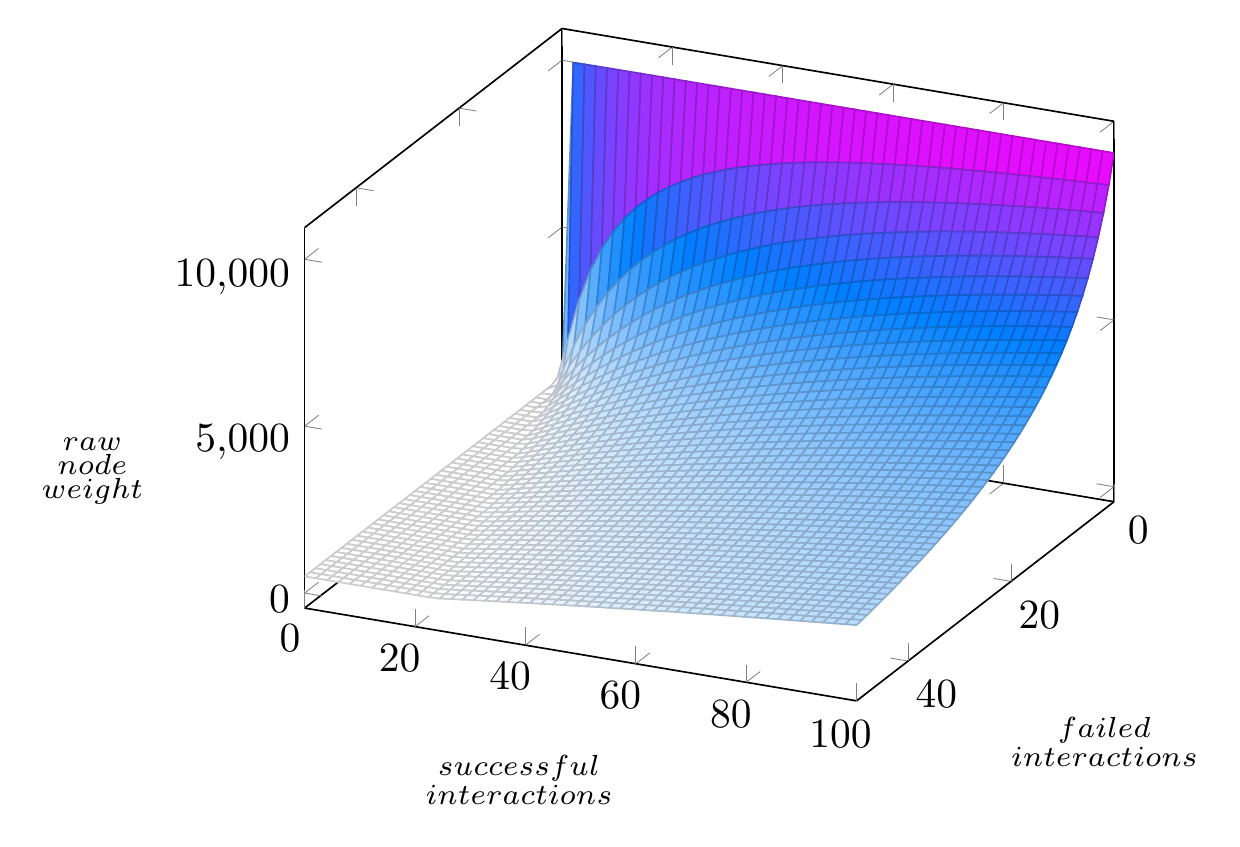
\begin{tikzpicture}[scale=1.5]
			\begin{axis}[
					scaled z ticks=false,
					colormap/cool,
					y dir=reverse,
					zlabel style={rotate=-90},
					xlabel = {$\substack{successful\\interactions}$},
					ylabel = {$\substack{failed\\interactions}$},
					zlabel = {$\substack{raw\\node\\weight}$}
				]
				\addplot3[surf, samples=50, domain=0:100, y domain=50:0] {max(500, x * 10000 / (x + 9 * y))};
			\end{axis}
		\end{tikzpicture}
	}{Raw Node Weight}
\end{figure}

\begin{align*}
\mathit{rawWeight} = \max\left(500, \frac{s \cdot 10000}{s + 9 \cdot f}\right)
\end{align*}
\end{itemize}

This formula guarantees that failed interactions rapidly decrease the weight of a remote node and its likelihood of getting selected.
The presence of a minimum score still gives a node with many failures a slight chance for being selected and possibly improving its score with more interactions.

The raw weight is multiplied with a weight multiplier to give the final weight of a node.
For static nodes, the multiplier is 2.
For dynamic nodes, it is 1.
If a node is banned due to consecutive interaction failures (see section \autoref{sec:reputation:NodeBanning}) , the multiplier is decreased by 1.
This ensures that a node does not connect to dynamic banned nodes.
The chance of connecting to static banned nodes is reduced by half.

Removal candidates are determined based on their connection age.
Each removal candidate that will be closed is replaced with a connection to a new node so that the node maintains the desired level of connections.
Finally, for each free slot, a candidate node has a chance of getting selected given by:

\begin{align*}
P(\textrm{node is getting selected}) = \frac{\textit{node weight}}{\sum\limits_{\substack{candidates\\nodes}} \textit{candidate node weight}}
\end{align*}

\subsection{Node Banning}
\index{reputation!node!banning}
\label{sec:reputation:NodeBanning}

In a public network there could be potentially malicious nodes that try to disturb normal processing of the network.
Therefore, if a node considers a remote node malicious, it will prevent connecting to that node and will not accept incoming connections from it.

Banning is applied at node level and is attached to a node's network scoped identifier \nemrefparens{sec:network:discovery}.
A misbehaving node will be immediately banned for a period of \nemsetting{node}{defaultBanDuration}.
Even after a node is no longer actively banned, the local node will remember for some time (\nemsetting{node}{keepAliveDuration}) that the node was behaving badly and treat repeat violations more severely by banning the node for longer time periods up to \nemsetting{node}{maxBanDuration}.
During banning, no connections with the banned node will be established.
After banning has expired, the node is treated like a normal interaction partner again.
There are various scenarios where a remote node will get banned.
The penalties vary based on the cause.

\makeatletter
\setlength{\@fptop}{0pt}
\makeatother
\begin{figure}[H]
	\nemcenterwithcaption{
		\begin{tabular}{|c|c|c|c|c|}
			\hline
			& \makecell{Connection\\closed} & \makecell{Remote\\can\\reconnect} & \makecell{Remote\\can be\\selected} & \makecell{Remote\\can send\\data}\\
			\hline
			\makecell{Consecutive\\interaction\\failures} & No & - & \makecell{Yes Static\\No Dynamic} & Yes\\
			\hline
			\makecell{Invalid\\data} & Yes & No & No & No\\
			\hline
			\makecell{Exceeded\\read rate} & Yes & No & No & No\\
			\hline
			\makecell{Unexpected\\data} & Yes & Yes & \makecell{Yes\\(after reconnect)} & \makecell{Yes\\(after reconnect)}\\
			\hline
		\end{tabular}
	}{Banning Rules}
\end{figure}

\subsubsection*{Consecutive Interaction Failures}
If interactions with the same node fail for too many consecutive times due to networking or stateful failures, it is better to suspend all interactions with that node for some time, hoping the node will behave better in the future.
The number of consecutive interaction failures before the node gets banned can be configured.
The amount of time the node gets banned is measured in selection rounds and can also be configured.
While the node is banned, it will not be actively selected as interaction partner, but it still can send new data.
This violation, therefore, only results in a partial ban.

\subsubsection*{Invalid Data}
Data can be invalid in many ways.
For example, if a remote node is on a fork, it might send a new block that does not fit into the local node's chain.
Little forks with a depth of one or two blocks happen frequently.
Though the sent data is invalid, it is not considered malicious because the remote node's internal state was understandably different.
On the other hand, sending data with invalid signatures clearly indicates that the remote node is malicious because signature verification is independent of a node's state.
The same is true for other verification failures that do not depend on the state of a node.
In all those cases, the remote node gets banned.

\subsubsection*{Exceeded Read Data Rate}
To prevent malicious nodes from spamming other nodes with excessive amounts of data, each node monitors the read rate from the socket used for communication.
If the data read during a configured time interval exceeds a maximum, the socket is closed and the node is banned.
The maximum read rate is configurable.

\subsubsection*{Unexpectedly Receiving Data}
There are situations during node communication where the local node is not expecting to receive any data from the remote.
If the remote still sends data in such a situation, it is violating the protocol and the connection is closed.
In this case, the connection is immediately closed but there is no persistent banning of the node.

	\section{Consensus}
\label{sec:consensus}

Aliquam sem fringilla ut morbi tincidunt. Et molestie ac feugiat sed lectus vestibulum. Leo vel fringilla est ullamcorper eget nulla facilisi. Pharetra convallis posuere morbi leo urna molestie at elementum. Mauris cursus mattis molestie a iaculis at. Sapien nec sagittis aliquam malesuada bibendum arcu. Consectetur adipiscing elit ut aliquam purus sit amet luctus. Egestas dui id ornare arcu. Nunc sed id semper risus in hendrerit gravida. Eu feugiat pretium nibh ipsum consequat nisl vel.

	\section{Time Synchronization}
\label{sec:timesync}

\nemquote{%
Time and Tide wait for no man.
}{Geoffrey Chaucer}

\nemchapterfirstletter{L}{ike} most other blockchains, \codenamespace relies on timestamps for transactions and blocks.
Ideally, all nodes in the network should be synchronized with respect to time.
Even though most modern operating systems have time synchronization integrated,
nodes can still have local clocks that deviate from real time by more than a minute.
This causes those nodes to reject valid transactions or blocks, which makes it impossible for them to synchronize with the network.

It is therefore needed to have a synchronization mechanism to ensure all nodes agree on time.
There are basically two ways to do this:
\begin{enumerate}
\item Use an existing protocol, such as NTP
\item Use a custom protocol
\end{enumerate}

The advantage of using an existing protocol like NTP is that it is easy to implement and the network time will always be near real time.
This has the disadvantage that the network relies on servers outside the network.

Using a custom protocol that only relies on the P2P network itself solves this problem, but there is a trade off.
It is impossible to guarantee that the network time is always near real time.
For an overview of different custom protocols see \cite{Scipioni2009}.
\codenamespace uses a custom protocol based on Chapter 3 of this thesis in order to be completely independent from any outside entity.
The protocol is implemented in the timesync extension.

\subsection{Gathering samples}
\index{time offset}

Each node in the network manages an integer \emph{offset} that is set to 0 at start.
The local system time in milliseconds adjusted by the offset (which can be negative) is the \nind{network time} (again in milliseconds) of the node.

After the start up of a node is completed, the node (hereafter called \emph{local node}) selects partner nodes for performing a time synchronization round.

For all selected partners, the local node sends out a request asking the partner for its current network time.
The local node remembers the network timestamps when each request was sent and when each response was received.
Each partner node responds with a sample that contains the timestamp of the arrival of the request and the timestamp of the response.
The partner node uses its own network time to create the timestamps.
\autoref{fig:timesync:img1} illustrates the communication between the nodes.

\begin{figure}
	\nemcenterwithcaption{
		\begin{figure}
\centering
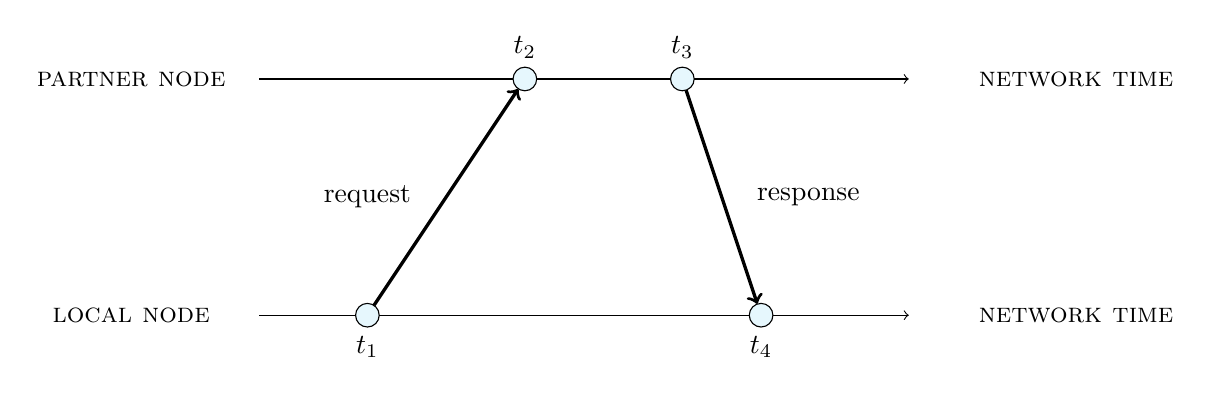
\begin{tikzpicture}[auto, thick, trans/.style={very thick,->}, time/.style={thin,->}]

%dummy nodes
\node[ctra] (l0) at (-1.5, -3) {};
\node[ctra] (l1) at (7, -3) {};
\node[ctra] (p0) at (-1.5, 0) {};
\node[ctra] (p1) at (7, 0) {};

\node[cblue,minimum size=1.5cm] (t1) at (0,-3) {};
\node[cblue,minimum size=1.5cm] (t2) at (2,0) {};
\node[cblue,minimum size=1.5cm] (t3) at (4,0) {};
\node[cblue,minimum size=1.5cm] (t4) at (5,-3) {};
 
 % Physical layer links
  \path[thin] (p0) edge (t2);
  \path[thin] (t2) edge (t3);
  \path[time] (t3) edge (p1);

  \path[thin] (l0) edge (t1);
  \path[thin] (t1) edge (t4);
  \path[time] (t4) edge (l1);

  \path[trans] (t1) edge (t2);
  \path[trans] (t3) edge (t4);
 
 % Legends
  \node[legend_normal] at (0, -3.4) {$t_1$};
  \node[legend_normal] at (2, 0.4) {$t_2$};
  \node[legend_normal] at (4, 0.4) {$t_3$};
  \node[legend_normal] at (5, -3.4) {$t_4$};

  \node[legend_normal] at (0, -1.5){request};
  \node[legend_normal] at (-3, -3){\textsc{local node}};
  \node[legend_normal] at (-3, 0){\textsc{partner node}};

  \node[legend_normal] at (5.6, -1.5){response};
  \node[legend_normal] at (9, -3){\textsc{network time}};
  \node[legend_normal] at (9, 0){\textsc{network time}};
\end{tikzpicture}

\caption{Communication between local and partner node.}
\label{fig:timesync}
\end{figure}

	}{Communication between local and partner node.\label{fig:timesync:img1}}
\end{figure}

Using the timestamps, the local node can calculate the round trip time
$$\mathvar{rtt} = (t_4 - t_1) - (t_3 - t_2)$$
and then estimate the offset o between the network time used by the two nodes as
$$o = t_2 - t_1 - \frac{\mathvar{rtt}}{2}$$

This is repeated for every time synchronization partner until the local node has a list of offset estimations.

\subsection{Applying filters to remove bad data}

There could be bad samples due to various reasons:
\begin{itemize}
\item A malicious node supplies incorrect timestamps.
\item An honest node has a clock far from real time without knowing it and without having synchronized yet.
\item The round trip time is be highly asymmetric due to internet problems or one of the nodes being very busy.
This is known as channel asymmetry and cannot be avoided.
\end{itemize}

Filters are applied that try to remove the bad samples. The filtering is done in three steps:
\begin{enumerate}
\item If the response from a partner is not received within an expected time frame (i.e. if $t_4-t_1 > 1000ms$) the sample is discarded.
\item If the calculated offset is not within certain bounds, the sample is discarded.
The allowable bounds decrease as a node's uptime increases.
When a node first joins the network, it tolerates a high offset in order to adjust to the already existing consensus of network time within the network.
As time passes, the node gets less tolerant with respect to reported offsets.
This ensures that malicious nodes reporting huge offsets are ignored after some time.
\item The remaining samples are ordered by their offset and then alpha trimmed on both ends.
In other words, on both sides a certain portion of the samples is discarded.
\end{enumerate}

\subsection{Calculation of the effective offset}

The reported offset is weighted with the importance of the boot account of the node reporting the offset.
Only nodes that expose a minimum importance are considered as partners in order to avoid solely picking nodes with nearly zero importance.
This is done to prevent Sybil attacks.

An attacker that tries to influence the calculated offset by running many nodes with low importances reporting offsets close to the tolerated bound will therefore not have a bigger influence than a single node having the same cumulative importance reporting the same offset.
The influence of the attacker will be equal to the influence of the single node on a macro level.

Also, the numbers of samples that are available and the cumulative importance of all partner nodes should be incorporated.
Each offset is therefore multiplied with a scaling factor.

Let $I_j$ be the importance of the node reporting the $j$-th offset $o_j$,
$n$ be the number of nodes that were eligible for the last PoI calculation and $s$ be the number of samples.

Then the scaling factor used is
$$ \mathvar{scale} = \min\left(\frac{1}{\sum_j I_j}, \frac{1}{\frac{s}{n}}\right)$$

This gives the formula for the effective offset $o$
$$ o = \mathvar{scale} \sum_j I_j \: o_j$$

Note that the influence of an account with large importance is artificially limited because the term $\frac{n}{s} $ caps the scale.
Such an account can raise its influence on a macro level by splitting its balance into accounts that are not capped.
But, doing so will likely decrease its influence on individual partners because the probability that all of its split accounts are chosen as time-sync partners for any single node is low.

\subsection{Coupling and threshold}

New nodes that just joined the network need to quickly adjust their offset to the already established network time.
In contrast, old nodes should behave a lot more rigid in order to not get influenced by malicious nodes or newcomers too much.

In order to enable this, nodes only adjust a portion of the reported effective offset.
Nodes multiply the effective offset with a coupling factor to build the final offset.

Each node keeps track of the number of time synchronization rounds it has performed.
This is called the node age.

The formula for this coupling factor $c$ is:
$$c = \max\left(\euler^{-0.3a},\: 0.1\right) \; \text{where} \; a = \max(nodeAge - 5,\: 0)$$

This ensures that the coupling factor will be 1 for 5 rounds and then decay exponentially to 0.1.

\begin{figure}
	\nemcenterwithcaption{
		\begin{tikzpicture}[trim axis left]
			\begin{axis}[
					scale only axis,
					xlabel = round,
					ylabel = coupling,
					height = 5cm,
					width=\textwidth / 2
				]
				\addplot[color=blue,domain=0.1:20,]{max(exp(-0.3*max(x-5, 0)), 0.1))};
			\end{axis}
		\end{tikzpicture}
	}{Coupling factor}
\end{figure}

Finally, a node only adds any calculated final offset to its internal offset if the absolute value is above a given threshold (currently set to 75ms).
This is effective in preventing slow drifts of the network time due to the communication between nodes having channel asymmetry.

	\section{Messaging}
\label{sec:messaging}

% custom message commands
\newcommand{\messagefield}[3]{
	\draw[] (0, #3 + 0.25) node[label=left:\small{#1}]{};
	\draw[draw=black] (0, #3) rectangle (4, #3 + 0.5);
	\draw[] (2, #3 + 0.25) node[label=center:\small{#2}]{};
}

\nemquote{
}{}

\nemchapterfirstletter{B}{lockchain} client applications retrieve blockchain data and present it to their users.
In order for these clients to be most useful, they should always present the most up to date blockchain data and refresh their user interfaces whenever the displayed data changes.
A naive client could periodically poll a REST server or a local database for blockchain data.
This is inefficient because it requires using more network bandwidth and other resources than necessary.
Instead, \codenamespace allows clients to subscribe to data changes via a single message queue.

\subsection{Message Channels And Topics}
\index{messaging!channels}
\label{sec:messaging:channels}

The \codenamespace message queue exposed to clients supports multiple channels.
Each channel has a unique \emph{topic}.
A topic always starts with a topic marker that indicates the kind of messages that will be received.
In some cases, the marker is followed by an unresolved address that is used for additional filtering.
Since a client is usually not interested in every type of blockchain state change, it can subscribe to a subset of available topics.
\autoref{tbl:messaging:topicMarkers} lists all supported topic markers.

\begin{figure}[H]
	\nemcenterwithcaption{
		\begin{tabular}{|l|c|}
			\hline
			\rule{0pt}{20pt}\textbf{Topic marker name} & \textbf{Topic marker}\\[1.2ex]
			\hline
			Block & 0x9FF2D8E480CA6A49\\
			\hline
			Drop blocks & 0x5C20D68AEE25B0B0\\
			\hline
			Transaction & 0x61\\
			\hline
			Unconfirmed transaction add & 0x75\\
			\hline
			Unconfirmed transaction remove & 0x72\\
			\hline
			Partial transaction add & 0x70\\
			\hline
			Partial transaction remove & 0x71\\
			\hline
			Transaction status & 0x73\\
			\hline
			Cosignature & 0x63\\
			\hline
		\end{tabular}
	}{Topic Markers}
	\label{tbl:messaging:topicMarkers}
\end{figure}

\subsection{Connection And Subscriptions}
\index{messaging!messages}
\label{sec:messaging:messages}

Support for messaging is added by the zeromq extension.
If a node wants to support messaging, this extension must be enabled in the broker process.
The extension registers subscribers for block and transaction related events \nemrefparens{sec:system:extensions} and maps those events to message queue messages.
When enabled, the broker listens on port \nemsetting{messaging}{subscriberPort} for new subscribers.
Clients can connect and subscribe to the message queue for one or more topics.

\subsection{Block Messages}

The topics for block messages only consist of a topic marker.
The layouts for all block messages are displayed in \autoref{fig:messaging:blockMessages}.
The following block messages are supported:

\begin{itemize}
	\item{Block: A new block was added to the chain.}
	\item{Drop blocks: Blocks after a given height were dropped.}
\end{itemize}

\begin{figure}[H]
	\nemcenterwithcaption{
		\begin{subfigure}{.5\textwidth}
			\begin{tikzpicture}[>=latex,font=\sffamily,semithick]
				\messagefield{0x00}{0x9FF2D8E480CA6A49}{0.0}
				\messagefield{0x08}{Block header}{-0.5}
				\messagefield{0x138}{Entity hash}{-1.0}
				\messagefield{0x158}{Generation hash}{-1.5}
			\end{tikzpicture}
			\caption{Block message layout}
		\end{subfigure}%
		\begin{subfigure}{.5\textwidth}
			\begin{tikzpicture}[>=latex,font=\sffamily,semithick]
				\messagefield{0x00}{0x5C20D68AEE25B0B0}{0.0}
				\messagefield{0x08}{Height}{-0.5}
			\end{tikzpicture}
			\caption{Drop blocks message layout}
		\end{subfigure}
	}{Block related messages}
	\label{fig:messaging:blockMessages}
\end{figure}

\subsection{Transaction Messages}

The topics for transaction messages consist of both a topic marker and an optional unresolved address filter.
When an unresolved address filter is supplied, only messages that involve the specified unresolved address will be raised.
For example, a message will be raised for a transfer transaction only if the specified unresolved address is the sender or the recipient of the transfer.
When no unresolved address filter is supplied, messages will be raised for all transactions.
The layouts for all transaction messages are displayed in \autoref{fig:messaging:unconfirmedTransactionMessages} , \autoref{fig:messaging:partialTransactionMessages} and \autoref{fig:messaging:transactionStatusMessage}.
The following transaction messages are supported:

\begin{itemize}
	\item{Transaction: A transaction was confirmed, i.e. is part of a block.}
	\item{Unconfirmed transaction add: An unconfirmed transaction was added to the unconfirmed transactions cache.}
	\item{Unconfirmed transaction remove: An unconfirmed transaction was removed from the unconfirmed transactions cache.}
	\item{Partial transaction add: A partial transaction was added to the partial transactions cache.}
	\item{Partial transaction remove: A partial transaction was removed from the partial transactions cache.}
	\item{Transaction status: The status of a transaction changed.}
\end{itemize}

\begin{figure}[H]
	\nemcenterwithcaption{
		\begin{subfigure}{.5\textwidth}
			\begin{tikzpicture}[>=latex,font=\sffamily,semithick]
				\messagefield{0x00}{0x75}{0.0}
				\messagefield{0x01}{Unresolved address}{-0.5}
				\messagefield{0x26}{Transaction T}{-1}
				\messagefield{0x26 + T::Size}{Entity hash}{-1.5}
				\messagefield{0x46 + T::Size}{Merkle component hash}{-2}
			\end{tikzpicture}
			\caption{Add message}
		\end{subfigure}%
		\begin{subfigure}{.5\textwidth}
			\begin{tikzpicture}[>=latex,font=\sffamily,semithick]
				\messagefield{0x00}{0x72}{0.0}
				\messagefield{0x01}{Unresolved address}{-0.5}
				\messagefield{0x26}{Entity hash}{-1.0}
			\end{tikzpicture}
			\caption{Remove message}
		\end{subfigure}%
	}{Unconfirmed transactions related messages}
	\label{fig:messaging:unconfirmedTransactionMessages}
\end{figure}

\begin{figure}[H]
	\nemcenterwithcaption{
		\begin{subfigure}{.5\textwidth}
			\begin{tikzpicture}[>=latex,font=\sffamily,semithick]
				\messagefield{0x00}{0x70}{0.0}
				\messagefield{0x01}{Unresolved address}{-0.5}
				\messagefield{0x26}{Transaction T}{-1}
				\messagefield{0x26 + T::Size}{Entity hash}{-1.5}
				\messagefield{0x46 + T::Size}{Merkle component hash}{-2}
			\end{tikzpicture}
			\caption{Add message}
		\end{subfigure}%
		\begin{subfigure}{.5\textwidth}
			\begin{tikzpicture}[>=latex,font=\sffamily,semithick]
				\messagefield{0x00}{0x71}{0.0}
				\messagefield{0x01}{Unresolved address}{-0.5}
				\messagefield{0x26}{Entity hash}{-1.0}
			\end{tikzpicture}
			\caption{Remove message}
		\end{subfigure}%
	}{Partial transactions related messages}
	\label{fig:messaging:partialTransactionMessages}
\end{figure}

\begin{figure}[H]
	\nemcenterwithcaption{
		\begin{subfigure}{.5\textwidth}
			\begin{tikzpicture}[>=latex,font=\sffamily,semithick]
				\messagefield{0x00}{0x73}{0.0}
				\messagefield{0x01}{Unresolved address}{-0.5}
				\messagefield{0x26}{Transaction status}{-1}
			\end{tikzpicture}
			\caption{Add message}
		\end{subfigure}%
	}{Transaction status message}
	\label{fig:messaging:transactionStatusMessage}
\end{figure}

\subsubsection{Cosignature Message}

The topic for a cosignature message consists of both a topic marker and an optional unresolved address filter.
The message is emitted to the subscribed clients when a new cosignature for an aggregate transaction is added to the partial transactions cache.
When an unresolved address filter is supplied, messages will only be raised for aggregate transactions that involve the specified address.
Otherwise, messages will be raised for all changes.
The layout for the cosignature message is displayed in \autoref{fig:messaging:cosignatureMessage}.

\begin{figure}[H]
	\nemcenterwithcaption{
		\begin{subfigure}{.5\textwidth}
			\begin{tikzpicture}[>=latex,font=\sffamily,semithick]
				\messagefield{0x00}{0x63}{0.0}
				\messagefield{0x01}{Unresolved address}{-0.5}
				\messagefield{0x26}{Signer public key}{-1}
				\messagefield{0x46}{Signature}{-1.5}
				\messagefield{0x86}{Aggregate hash}{-2}
			\end{tikzpicture}
		\end{subfigure}%
	}{Cosignature message}
	\label{fig:messaging:cosignatureMessage}
\end{figure}


	\printbibliography[heading=bibintoc]

	\printindex
\end{CJK}
\end{document}
